%% =====================================================================
%%  Savana -- first full draft targeting USENIX Security '27
%%
%%  Build (Overleaf or local): pdfLaTeX, main document = main.tex,
%%  bibliography = BibTeX.  If the official USENIX style file
%%  usenix-2020-09.sty is present it is used; otherwise the bundled
%%  usenix-fallback.sty approximates the layout (NOT for submission).
%%
%%  Status (2026-10-07): design and implementation sections are written
%%  against the source at the evaluated commit (claims audited against
%%  code; see the draft README).  The evaluation reports measured
%%  results; items still open are marked TODO / TBD.  Search for
%%  "TODO" before submission.
%% =====================================================================
\documentclass[letterpaper,twocolumn,10pt]{article}

\IfFileExists{usenix-2020-09.sty}{\usepackage{usenix-2020-09}}{\usepackage{usenix-fallback}}

\usepackage{amsmath,amssymb}
\usepackage{booktabs}
\usepackage{array}
\usepackage{tabularx}
\usepackage{multirow}
\usepackage{graphicx}
\usepackage{enumitem}
\usepackage{listings}
\usepackage{xcolor}
\usepackage{url}
\usepackage{tikz}
\usetikzlibrary{arrows.meta,positioning,fit,calc,shapes.geometric}

% ---------------------------------------------------------------------
% Submission switches
% ---------------------------------------------------------------------
\newif\ifanonymous
\anonymoustrue            % USENIX Security submissions are double-blind

% ---------------------------------------------------------------------
% Macros
% ---------------------------------------------------------------------
\newcommand{\sys}{Savana}
\newcommand{\code}[1]{\texttt{\detokenize{#1}}}
\newcommand{\todo}[1]{{\color{red}\textbf{[TODO: #1]}}}
\newcommand{\tbd}{{\color{red}TBD}}
\newcommand{\pending}[1]{{\color{blue!60!black}\textit{#1}}}
\newcommand{\lbl}[4]{\ensuremath{\langle #1,\,#2,\,#3,\,#4\rangle}}
\newcommand{\READ}{\textsc{read}}
\newcommand{\SEND}{\textsc{send}}
\newcommand{\integ}{\mathit{int}}
\newcommand{\conf}{\mathit{conf}}
\newcommand{\readers}{\mathit{readers}}
\newcommand{\effects}{\mathit{effects}}
\newcommand{\join}{\sqcup}
\newcommand{\camel}{CaMeL}
\newcommand{\camelp}{CaMeL+policy}

\lstdefinelanguage{Rust}{
  morekeywords={fn,let,match,pub,const,impl,enum,struct,Some,None,Ok,Err,return,if,else,for,in,mut,use,mod,trait,where,as,ref,self,Self},
  sensitive=true,
  morecomment=[l]{//},
  morecomment=[s]{/*}{*/},
  morestring=[b]",
}
\lstset{
  basicstyle=\ttfamily\scriptsize,
  columns=fullflexible,
  keepspaces=true,
  breaklines=true,
  frame=single,
  framerule=0.3pt,
  xleftmargin=4pt,
  xrightmargin=4pt,
  aboveskip=6pt,
  belowskip=6pt,
  language=Rust,
  keywordstyle=\bfseries,
  commentstyle=\color{black!55},
}

\setlist{nosep,leftmargin=*}

% ---------------------------------------------------------------------
\begin{document}

\date{}

\title{\Large \bf \sys{}: Confining Disclosure and Effects in LLM Agents\\
  \large When the Planner Is Not Trusted Either}

\ifanonymous
\author{
  {\rm Anonymous Author(s)}\\
  Submission to USENIX Security '27
}
\else
\author{
  {\rm Author Names}\\
  Author Affiliations
}
\fi

\maketitle

% =====================================================================
\begin{abstract}
Tool-using large language model (LLM) agents read attacker-controlled
content and act with a user's authority. System-level defenses such as
CaMeL separate a privileged planner from untrusted data, but they still
trust the planner: whatever the plan writes is authorized. We present
\sys{}, a security kernel that treats every model, the planner included, as
an untrusted proposer. The user (the \emph{owner}) signs a task authority
with one clause per operation, and the kernel binds every argument of every
dispatched tool call to an origin: owner text, an owner-declared constant,
or a value the kernel itself derived along an owner-signed edge from an
earlier authorized result. Disclosure is mediated by four-dimensional
information-flow labels and signed, recipient-bound declassification, and
every effect is journaled before its first byte leaves the system.

We implement \sys{} as five mutually authenticated Rust services. On all
949 injection pairs of AgentDojo~v1.2.2, \sys{} admits no targeted attack and
no unauthorized tool request, whereas CaMeL with the same model admits 2.
When the planner itself is given hidden attacker objectives, the same model
inside CaMeL executes 7 recipient redirections and at least 3 value changes
(3 and 2 under CaMeL's policies); inside \sys{} it executes none, and every
attempt is refused before signing. A value-blind planner sees none of the
owner's personal data. The cost is utility: \sys{} completes 40 of 97 benign
tasks (41 with deterministic compute steps), against 58 for CaMeL (39
with its policies). We attribute every remaining failure; the largest share
follows directly from refusing destinations chosen by data.
\end{abstract}

% =====================================================================
\section{Introduction}
\label{sec:intro}

LLM agents combine a model with tools that read data and change external
state. This creates a confused-deputy problem: web pages, documents,
e-mail, and tool results are attacker-influenced, yet they enter the same
model context that drives action selection. Prompt injection exploits this
ambiguity to turn data into instructions~\cite{perez2022ignore,greshake2023}.
Instruction hierarchies, input transformations, and alignment reduce attack
success~\cite{wallace2024hierarchy,hines2024spotlighting,chen2025struq,chen2025secalign},
but they leave the model on the authorization path, and adaptive attacks
routinely break them~\cite{nasr2026attacker}.

Systems security answers confused deputies by separating decision-making from
authority~\cite{saltzer1975,dennis1966,miller2006robust}: untrusted components
may compute over data, but a reference monitor decides which principals may
observe a value and which effects it may
authorize~\cite{denning1976,myers1997,efstathopoulos2005,zeldovich2006,krohn2007}.
CaMeL~\cite{debenedetti2025camel} brought this idea to agents. A privileged
LLM (P-LLM) sees only the user's query and writes a program; a quarantined
LLM processes untrusted data; an interpreter tracks capabilities and checks
policies before each tool call. Follow-up systems refine the planner, the
policies, or the isolation~\cite{costa2025fides,shi2025progent,li2025drift,ace2026,ipiguard2025}.

These designs share one trust assumption: the planner's output is the user's
intent. A literal the P-LLM writes into its program is treated as trusted,
because the P-LLM saw only the user's query. That assumption fails when the
planner itself is compromised---by a malicious or backdoored model provider,
by a poisoned fine-tune, or by an injection that reaches it through
conversation history or memory. We measured what this means in practice
(\S\ref{sec:eval-planner}). We gave the same model, used as CaMeL's P-LLM, a
hidden objective to redirect the user's sends to an attacker. Over 97
benign AgentDojo tasks, CaMeL executed 7 writes that included the attacker:
it added the attacker as a meeting participant, shared a file with the
attacker, and copied the attacker on an e-mail. Three of these runs were
still scored as successful by the benchmark, because the official task
checker does not look for an extra recipient. CaMeL's policies blocked
four, but only because the same policies already reject those tasks for
an honest planner. They admitted the other three, because the attacker's
address was a literal in trusted code.

\sys{} takes the next step: \emph{no model is on the authorization path,
including the one that writes the plan.} Three challenges follow.
\begin{description}[style=nextline,font=\bfseries]
\item[C1: Authority without a trusted planner.] If the plan is untrusted,
  something else must say which tools may run, against which resources and
  destinations, and with which values.
\item[C2: Data-dependent tasks.] Real tasks need values found in data: an
  IBAN in a bill, the highest-rated hotel, the end time of a meeting. These
  values must be able to fill a field without being able to choose an
  effect.
\item[C3: Mediated disclosure and durable effects.] Every model, approver,
  and executor sees only what policy admits; and the decision to act must
  survive policy changes and crashes without duplicating an effect whose
  outcome is unknown.
\end{description}

\sys{} answers C1 with an owner-signed \emph{task authority}: one clause per
operation, fixing the tool, its effect, resource, destination, and bounds.
The planner proposes a whole program over a reviewed catalog. A fixed owner
review admits or refuses it, but the review is only a pre-filter; the kernel
is the reference monitor. For C2, a value may come from data only along an
owner-signed \emph{edge}: the kernel itself extracts it from an earlier
authorized result, at a signed JSON path, within a signed byte bound, or
through a quarantined extractor or a deterministic computation the owner
named. Such a value carries untrusted integrity and can never be a
destination. For C3, \sys{} labels every value along four dimensions
(integrity, confidentiality, readers, effects), admits audience expansion
only through signed and recipient-bound declassification transitions, and
journals every effect before its first provider byte.

\paragraph{Results.} On AgentDojo~v1.2.2~\cite{debenedetti2024agentdojo}
with DeepSeek models, every batch ran on a fresh, disposable host, and
every batch passed offline re-verification of its evidence chain.
\begin{itemize}
\item \textbf{Injections:} \sys{} admitted no targeted attack and no
  unauthorized tool request across all 949 injection pairs. CaMeL with the
  same model admitted 2, both of which push a hotel recommendation through
  the answer text, which is outside \sys{}'s structural guarantee
  (\S\ref{sec:eval-injection}).
\item \textbf{Compromised planner:} the planner was given four hidden
  attacker objectives, across 388 episodes plus 194 more with up to three
  drafts. No attacker effect and no unauthorized request occurred. Every
  program that encoded an attack was refused before it was signed.
\item \textbf{Privacy:} the value-blind planner and extractor reduce the
  personal data that models receive from 27 and 1,093 detected spans to
  zero.
\item \textbf{Utility:} \sys{} completes 40/97 benign tasks, or 41/97
  with deterministic compute steps, against 58 for CaMeL and 39 for CaMeL
  with its policies. With a stronger model, CaMeL rises to 71 and 47;
  \sys{} does not improve. Five banking tasks pass even if the agent does
  nothing; we report scores with and without them.
\end{itemize}
We attribute every failure. Most follow from two deliberate choices:
recipients chosen by data are refused, and a task must complete within a
short authorization window.

\paragraph{Contributions.}
\begin{enumerate}
\item A security-kernel design in which the planner is outside the trusted
  computing base. An owner-signed task authority and per-value origin
  enforcement replace trust in the plan. Labels with an untrusted-effect
  ceiling and control-facet endorsement prevent data or planner choice
  from minting authority (\S\ref{sec:labels}, \S\ref{sec:programs}).
\item Owner-signed result edges that let data-dependent tasks run without
  giving data control. The edges cover JSON paths, typed lists,
  owner-stated computations, a quarantined extractor, conditional writes,
  and deterministic compute steps (\S\ref{sec:programs}).
\item Signed, recipient-bound declassification and journal-before-effect
  execution, implemented in five mutually authenticated services
  (\S\ref{sec:declass}--\S\ref{sec:impl}).
\item An evaluation of these mechanisms and of CaMeL under the same model,
  covering the full AgentDojo injection matrix, a compromised planner, model
  privacy, utility attribution, and cost (\S\ref{sec:eval}).
\end{enumerate}

% =====================================================================
\section{Background and Motivation}
\label{sec:background}

\subsection{Agents, tools, and planners}

An agent receives a request from its user, calls tools that read or change
external state, and returns an answer. Tool results---e-mails, files, web
pages, transaction histories---are written by third parties. An indirect
prompt injection places instructions in such a result. The goals are either
to \emph{disclose} data to an attacker-chosen sink, or to perform an
\emph{effect} the user did not request~\cite{greshake2023,debenedetti2024agentdojo}.

Plan-then-execute defenses fix the control flow before any untrusted data
is read. In CaMeL~\cite{debenedetti2025camel}, the P-LLM translates the
query into Python. Tool results are opaque values tagged with
capabilities, and a quarantined LLM can turn them into structured values
but cannot call tools. Security policies are checked before each tool
call. In the reference implementation they are applied by replaying a
recorded run. Variants plan over abstract tools (ACE~\cite{ace2026}),
build tool-dependency graphs (IPIGuard~\cite{ipiguard2025}), learn
privilege policies (Progent~\cite{shi2025progent}), or label values with
information-flow types (FIDES~\cite{costa2025fides}).

\subsection{The planner is an authorization input}

Table~\ref{tab:approaches} separates useful defenses from the property
\sys{} targets. A plan-then-execute design removes data from the control
path, but it keeps the planner on the \emph{authorization} path. Every
literal the P-LLM writes is an endorsed value. A recipient it invents is
indistinguishable from one the user named. This is a deliberate trust
choice. It is not a bug: the P-LLM saw only the query. But it makes the
planner's integrity part of the security argument.

\paragraph{Worked example A.} The user asks: \emph{``Please reschedule my
Dental check-up to 2024-05-20 at 10:00.''} We gave the same planner model a
hidden instruction to change amounts and times. Inside CaMeL, the
P-LLM wrote
\code{reschedule_calendar_event(event_id, "2024-05-21 11:00")}. The call
ran with and without CaMeL's policies, because the literal is trusted
code. Inside \sys{}, the same model drafted the same value. The owner
review refused the program before signing, because \code{2024-05-21 11:00}
is not text from the request and is not a value the owner declared. No
operation ran (\S\ref{sec:eval-planner}).

\begin{table}[t]
\centering\footnotesize
\begin{tabularx}{\columnwidth}{@{}p{0.22\columnwidth}p{0.28\columnwidth}X@{}}
\toprule
\textbf{Mechanism} & \textbf{What it addresses} & \textbf{Residual authority path}\\
\midrule
Instruction hierarchy~\cite{wallace2024hierarchy} & Conflicting instructions & Model output remains an authorization input.\\
Input/output detection~\cite{hines2024spotlighting,liu2024formalizing} & Known attack patterns & A missed attack reaches the same action path.\\
Tool isolation~\cite{wu2025isolategpt} & Tool-code compromise & Authorized arguments may still encode an unsafe effect.\\
Plan-then-execute~\cite{debenedetti2025camel,ace2026} & Data-driven control flow & The planner's literals and tool choices are trusted.\\
Human approval & User consent & Security depends on who constructs the displayed bytes.\\
\midrule
\sys{} & Disclosure and effect mediation & No model output carries a capability; every value has a signed origin.\\
\bottomrule
\end{tabularx}
\caption{Defense mechanisms are complementary. \sys{} moves authorization
out of every model, including the planner, and mediates disclosure and
effects at a reference monitor.}
\label{tab:approaches}
\end{table}

% =====================================================================
\section{Threat Model and Goals}
\label{sec:threat}

\subsection{Adversary}

The adversary controls all content the agent reads: web pages, documents,
messages, and tool results. It may choose \emph{arbitrary output for every
model}: the planner that drafts the program, the quarantined extractor that
reads data, and any remote model. This covers prompt injection, a
malicious or backdoored model provider, and a planner with a hidden
objective. The adversary may gain arbitrary code execution in the agent
daemon. It may operate a registered connector and control the bytes that
connector returns. It also controls the network: it may observe, delay,
replay, reorder, modify, or drop messages. We separately inject crash
faults at adversarially chosen instruction and durability boundaries. The
adversary knows the design, the review rules, the catalog, and the prompts.

The adversary does not initially possess deployment, policy, service, owner,
or WebAuthn signing keys. It cannot break the cryptographic primitives, and
it cannot compromise the host kernel, hypervisor, or hardware root of trust.
Denial of service is always possible: an agent, model, connector, executor,
or network adversary may refuse to make progress.

\subsection{Trusted computing base}

\sys{} has a distributed, least-privilege TCB.
\begin{itemize}
\item The \textbf{owner} is trusted for intent. It states the request and
  signs the task authority. In our evaluation, a fixed review procedure acts
  for the owner: it admits or refuses a drafted program and is listed in the
  TCB (Table~\ref{tab:tcb}).
\item The \textbf{kernel} is trusted to enforce labels, provenance, value
  origins, policy, and dispatch state.
\item The \textbf{approval service} is trusted to authenticate the owner and
  to sign only a confirmation bound to the bytes rendered in its
  authenticated UI channel.
\item The \textbf{executor} is trusted to use connector credentials only for
  a kernel-authorized envelope, and to journal before crossing the
  external-byte boundary.
\item The \textbf{signing authorities} for deployment and declassification,
  the platform's cryptography, and process/IPC isolation are trusted.
\end{itemize}
\emph{No language model is trusted.}

Compromising a trusted component invalidates the property it owns. A
compromised executor can misuse connector credentials, so it is inside the
effect TCB. Mutual authentication prevents that compromise from also minting
kernel policy or approval settlements. This is compartmentalized trust, not
Byzantine fault tolerance.

Table~\ref{tab:tcb} gives a conservative crate-level accounting at the
evaluated commit. It counts complete crates, including inline tests and code
not exercised by every property, so it over-approximates the executable
slice.

\begin{table}[!h]
\centering\footnotesize
\begin{tabularx}{\columnwidth}{@{}XrX@{}}
\toprule
\textbf{Trusted component group} & \textbf{LOC} & \textbf{Properties}\\
\midrule
Kernel policy path (Rust) & 261{,}848 & S1--S6; policy-core, kerneld, protocol, vault, leak gate, input runtime\\
Approval service (Rust) & 18{,}235 & S1 for owner-endorsed actions\\
Executor (Rust) & 19{,}525 & S1 and S4 at the external-byte boundary\\
Platform identity (Rust) & 13{,}003 & service identity and process isolation\\
Owner review (Python) & ${\approx}$950 & S6 pre-filter in the evaluated deployment\\
\midrule
Conservative union & ${\approx}$313k & property-dependent distributed TCB\\
\bottomrule
\end{tabularx}
\caption{Conservative TCB accounting (physical lines, inline tests
included). The union is not the TCB of every request; each property relies
on the components named in its row.}
\label{tab:tcb}
\end{table}

\subsection{Security goals}

\begin{description}[style=nextline,font=\bfseries]
\item[S1 Effect authorization.] Every side effect corresponds to an
  exact-action capability prepared under the active signed policy. The
  capability is justified either by an owner-signed task clause matched in
  full, or by a matching single-use approval settlement.
\item[S2 Disclosure confinement.] A value crosses a reader boundary only if
  its label already admits that reader, or an authorized declassification
  transition admits the exact outgoing bytes.
\item[S3 No authority from untrusted data or choice.] A value with
  external-untrusted integrity carries no effect beyond \READ, including
  after derivation with a more trusted value. A planner's selection on any
  of seven control facets is recorded against the planner's output and
  re-checked before dispatch.
\item[S4 Recoverable attribution.] Every value and authorization decision is
  linked to bounded provenance and durable evidence. After a crash, the
  system distinguishes proven no-effect from an indeterminate effect, and
  never retries the latter automatically.
\item[S5 Fail-closed mediation.] Parse, verification, policy, gate,
  identity, freshness, and recovery failures do not widen readers or
  effects.
\item[S6 Origin confinement.] For every dispatched operation and for the
  final release, the tool, its effect, resource, destination, and bounds
  are fixed by an owner-signed clause. Every argument value is one of:
  (a) owner text, i.e.\ a substring of the request after NFC normalization
  and whitespace folding; (b) an owner-declared constant; or (c) a value
  the kernel derived along an owner-signed edge from an
  already-authorized result, within the signed path, byte bound, list form,
  and computation.
\end{description}

S2 is a mediation property, not a claim that a heuristic recognizes every
semantic secret. For model-facing declassification, the confidentiality
claim is parameterized by the deterministic sensitive-content predicate of
\S\ref{sec:gate}. S1, S3, and S6 do not depend on recognizing an injected
instruction. A missed instruction may change a model's proposal, but it does
not give that proposal a capability.

\subsection{Non-goals}

\sys{} does not make model output correct or useful. It does not protect
the \emph{wording} of a final answer that the owner asked a model to compose
from untrusted data. It does not tolerate compromise of the relevant TCB
component, and it does not resist timing or microarchitectural side
channels. It does not hide the structure of a plan from the planner that
wrote it. It does not control data after a correctly authorized release,
and it does not provide availability against a component that refuses
service. Within the owner's grant, a compromised planner may still choose
among owner-authorized values: for example, it may pick a different record
returned by the same authorized read. We measure this residue
(\S\ref{sec:eval-planner}) and do not claim to remove it.

% =====================================================================
\section{Overview}
\label{sec:overview}

\begin{figure}[t]
\centering
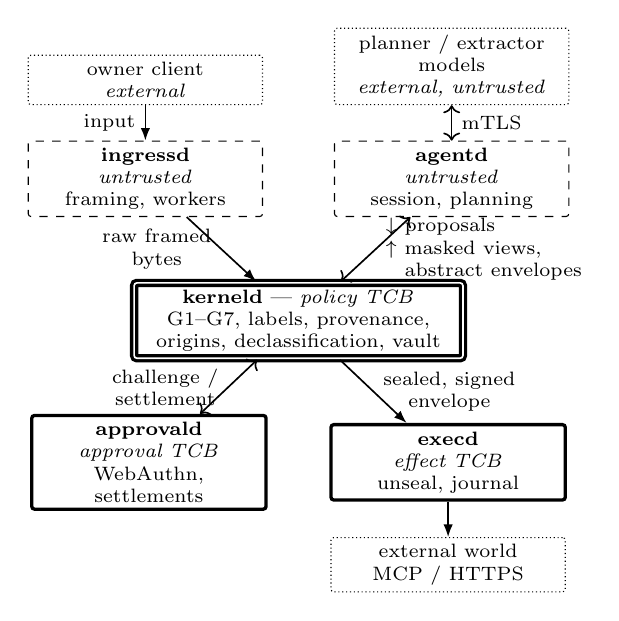
\begin{tikzpicture}[
  font=\scriptsize,
  node distance=4.5mm and 9mm,
  box/.style={draw,rounded corners=1pt,align=center,inner sep=2.5pt,minimum height=6mm,text width=28mm},
  untrusted/.style={box,dashed},
  policytcb/.style={box,double,very thick,text width=40mm},
  narrowtcb/.style={box,very thick},
  ext/.style={box,densely dotted},
  arr/.style={-{Latex[length=1.6mm]},semithick},
]
\node[untrusted] (ing) {\textbf{ingressd}\\\emph{untrusted}\\framing, workers};
\node[untrusted,right=of ing] (ag) {\textbf{agentd}\\\emph{untrusted}\\session, planning};
\node[ext,above=of ing] (br) {owner client\\\emph{external}};
\node[ext,above=of ag] (pl) {planner / extractor\\models\\\emph{external, untrusted}};
\node[policytcb] (k) at ($(ing)!0.5!(ag)+(0,-18mm)$) {\textbf{kerneld} --- \emph{policy TCB}\\G1--G7, labels, provenance,\\origins, declassification, vault};
\node[narrowtcb] (ap) at ($(k)+(-19mm,-18mm)$) {\textbf{approvald}\\\emph{approval TCB}\\WebAuthn, settlements};
\node[narrowtcb] (ex) at ($(k)+(19mm,-18mm)$) {\textbf{execd}\\\emph{effect TCB}\\unseal, journal};
\node[ext,below=of ex] (world) {external world\\MCP / HTTPS};
\draw[arr] (br) -- node[left,pos=.5]{input} (ing);
\draw[arr,<->] (ag) -- node[right,pos=.5]{mTLS} (pl);
\draw[arr] (ing) -- node[left,pos=.5,align=center]{raw framed\\bytes} (k);
\draw[arr,<->] (ag) -- node[right,pos=.5,align=left]{$\downarrow$ proposals\\$\uparrow$ masked views,\\\phantom{$\uparrow$} abstract envelopes} (k);
\draw[arr,<->] (k) -- node[left,pos=.5,align=center]{challenge /\\settlement} (ap);
\draw[arr] (k) -- node[right,pos=.5,align=center]{sealed, signed\\envelope} (ex);
\draw[arr] (ex) -- (world);
\end{tikzpicture}
\caption{Process decomposition, readable without color. Dashed boxes are
untrusted, dotted boxes are external, the double box owns policy, and thick
boxes are narrow TCB components for approval and effects. Each edge is a
distinct mutually authenticated Suite-1 channel.}
\label{fig:arch}
\end{figure}

\subsection{Process decomposition}

\sys{} is a multi-daemon system (Figure~\ref{fig:arch}). Isolation is a
property of process boundaries, not module boundaries: a compromised role
cannot assume another role's authority, because it does not hold that
role's keys or socket credentials.
\begin{itemize}
\item \code{savana-agentd} owns agent sessions and planner orchestration. It
  is untrusted by design.
\item \code{savana-ingressd} is the entry point for all owner input. It
  frames the bytes and runs parsers in disposable, sandboxed one-job
  workers.
\item \code{savana-kerneld} owns labels, provenance, value origins,
  declassification, the policy gates, and the vault.
\item \code{savana-approvald} owns WebAuthn credentials and signed approval
  settlements.
\item \code{savana-execd} owns connector credentials, effect dispatch, and
  the durable execution journal.
\end{itemize}
A trusted control shell can create tasks and read closed public status, but
receives no content and holds no data-plane key.

Eight inter-process edges exist. Each has a distinct client key, server
key, peer rule, endpoint role, and operation enumeration. There is no
control-shell-to-kernel, control-shell-to-executor, agent-to-executor, or
ingress-to-executor data-plane edge. Every edge uses \emph{Suite-1}:
\begin{itemize}
\item a fixed 16-byte handshake prefix and an ephemeral X25519 exchange;
\item an Ed25519-signed handshake transcript that binds both peers' process
  boot identifiers and the observed OS peer identity;
\item HKDF-SHA-256 traffic keys with mutual HMAC confirmation;
\item ChaCha20-Poly1305 records, with exactly one encrypted request and one
  encrypted response per connection.
\end{itemize}

\subsection{Two enforcement paths}

\paragraph{Interactive actions.} An agent proposes a tool class and
argument handles. The kernel resolves the class against the active signed
registry, matches the action against the owner's task authority, and
records the planner's choice on each of seven control facets
(\S\ref{sec:endorsement}). G5 validators then decide whether the action is
permitted or needs approval. G6 settles an approval, and G7 declassifies
the execution envelope, re-checks the endorsements against the current
state, and prepares the effect durably.

\paragraph{Owner-signed task programs.} This is the path we evaluate. The
planner drafts a whole program before any data is read (\S\ref{sec:programs}).
\begin{enumerate}
\item The owner signs a task authority with one clause per operation, plus
  a final release.
\item Signed operator commands compile the program against those clauses
  and prepare it. Preparation checks the origin of every input value
  \emph{before any operation runs}.
\item The kernel then drives the operations itself, one at a time, through
  the same G4--G7 path. Values taken from earlier results are minted only
  by the kernel.
\end{enumerate}
In both paths the agent and the planner hold no capability-bearing
credential, no stored plaintext, and no tool transport.

The implementation assigns these checks to seven gates:
\begin{itemize}
\item G1, input normalization;
\item G2, local semantic extraction;
\item G3, labels and declassification;
\item G4, matching the action against the task authority and binding it;
\item G5, internal validators;
\item G6, human approval;
\item G7, durable execution and recovery.
\end{itemize}
Each gate has a closed request vocabulary. No generic ``invoke handler''
operation crosses a service boundary.

\subsection{Security argument}

We state the argument over a durable event trace $\tau$. The relevant
events are:
\begin{itemize}
\item value construction and derivation;
\item a \emph{reveal} of exact bytes to a reader;
\item preparation of an exact-action capability;
\item the executor's first provider byte;
\item recovery classification.
\end{itemize}

\begin{description}[style=nextline,font=\bfseries]
\item[P1 Label closure.] Every ordinary derivation is non-widening in
  readers and effects, and every externally untrusted value satisfies the
  \READ-only ceiling.
\item[P2 Mediated disclosure.] (a) \emph{Reveals.} If $\tau$ reveals bytes
  $b$ of value $v$ to a system reader $r$ (a component or an exact model,
  executor, or sink identity), then either $r\in\readers(v)$ before the
  reveal, or $\tau$ contains an earlier declassification node for the same
  bytes, rule set, purpose, and recipient. (b) \emph{Releases through
  effects.} If action $a$ carries bytes $b$ to its external destination
  $d$, then $d$ is the owner-endorsed \textsf{Destination} facet of $a$,
  the bytes reached the executor through \textsf{BuildExecutionEnvelope}
  for $a$'s exact executor, and, if any argument of $a$ is
  \textsf{ExternalUntrusted} or $d$ was chosen by such a value, $\tau$
  contains a verified \textsf{ActionApproval} over $a$'s exact request
  bytes (\S\ref{sec:effect-readers}).
\item[P3 No data- or selection-derived authority.] An externally untrusted
  value may occur as an argument, but it cannot by itself justify a control
  facet or authorize an effect. For every dispatched action, $\tau$
  contains (i) the seven control selections, recorded against the
  planner's committed output, and (ii) endorsements that were re-checked
  against the current state immediately before durable preparation.
\item[P4 Authorized emission.] If the executor emits the first provider
  byte for action $a$, $\tau$ contains an earlier capability and durable
  preparation for the same action digest, executor, manifest, fence epoch,
  and execution nonce.
\item[P5 Crash containment.] For one execution nonce, the executor opens
  at most one provider attempt. After a crash past the first provider byte,
  the outcome is effect-started or indeterminate, and \sys{} never retries
  it automatically.
\item[P6 Origin confinement.] For every operation of an owner-signed
  program, each argument the executor receives equals one of three things:
  an owner-text item, an owner-declared constant, or the kernel's own
  derivation along the signed edge for that argument. In the third case,
  the derivation is taken over the retained result of an earlier operation
  of the same authority.
\end{description}

P1 follows by induction over the closed value constructors. P2(a) reduces
every reader-widening route to the private declassification constructor;
P2(b) reduces to the \textsf{Destination} endorsement and to G5's
fail-closed floor (\S\ref{sec:endorsement}).
P3 reduces each facet to its selection record and the endorsement re-check
at G7. P4 and P5 reduce the external-byte boundary to the kernel and
executor journals (\S\ref{sec:pipeline}). P6 reduces to two checks.
\begin{itemize}
\item \textbf{Preparation} runs the owner-text origin check before
  anything executes, and the result-edge rule: the owner's exact values,
  plus the declared edge rules, must reconstruct an alternative the owner
  signed.
\item \textbf{Dispatch} re-matches each request against its clause, where
  a result-derived value can be produced only by the kernel's own result
  derivation.
\end{itemize}
These are implementation arguments, not a mechanized proof
(\S\ref{sec:discussion}).

\subsection{P3 as robustness against an untrusted decider}
\label{sec:robustness}

P2 and P3 are instances of a property studied for two decades in
language-based security. \emph{Robust declassification}~\cite{zdancewic2001robust}
requires that an attacker who controls low-integrity inputs cannot
influence \emph{what} information is released. \emph{Qualified
robustness}~\cite{myers2006qualified} relaxes this to allow untrusted data to
affect a release only through an explicit endorsement, and
\emph{nonmalleable IFC}~\cite{cecchetti2017nmifc} adds the dual,
\emph{transparent endorsement}: a principal may only endorse information it
can read. Askarov and Myers characterize both in terms of attacker
control~\cite{askarov2011}; Sabelfeld and Sands classify release policies by
\emph{who}, \emph{what}, \emph{where}, and \emph{when}~\cite{sabelfeld2009declass}.

We use the same vocabulary. The \emph{decision} of an action consists of
its seven control facets and, for any action that releases data, its
recipient. P3 says that no low-integrity input---and here every model output
is low-integrity---influences that decision except through owner evidence:
\begin{itemize}
\item \textsf{ExplicitAlternative} and \textsf{CompleteContractSingleton} are
  decisions the owner made \emph{before} any untrusted byte was read: the
  candidate domain is the signed clause and nothing else
  (\S\ref{sec:completeness}). They correspond to robust declassification,
  where the release point and its policy are fixed in trusted code.
\item \textsf{ActionApproval} is an endorsement of exact bytes on an
  authenticated display. It corresponds to qualified robustness, and the
  display transition (\textsf{BuildApprovalDisplay}) makes it
  \emph{transparent}: the owner endorses only bytes it has been shown.
\end{itemize}

\paragraph{What is new.} Classical robustness assumes that the program is
trusted and the attacker controls only some of its inputs; the release
points are written by the programmer. In an agent, the ``program'' is a
plan written by a model, and we assume that model is the attacker. Three
consequences follow, and they are the parts of the design that the
classical results do not provide.
\begin{enumerate}
\item \textbf{The code is an input.} Robustness must hold when the
  attacker also chooses \emph{which} release points exist. \sys{} therefore
  never lets a release point originate in model output. The owner signs
  the program's control skeleton (the task authority), and every planner
  choice is recorded as a selection fixed at \textsf{ExternalUntrusted}
  and \READ, which no derivation can consume.
\item \textbf{Robustness is enforced dynamically, per action, and across
  restarts.} The kernel re-checks endorsements against the current
  authorization revision, pre-state, and candidate-domain digest
  immediately before durable preparation. A type system checks robustness
  once, at compile time; we must check it at the moment of effect, against
  durable state that an adversary can try to race or replay.
\item \textbf{Effects are releases.} An effect discloses its arguments to
  its destination. We treat the destination of every effect as a reader
  (\S\ref{sec:effect-readers}), so the same robustness condition governs
  both \emph{what} leaves (P2) and \emph{what happens} (P3).
\end{enumerate}

% =====================================================================
\section{Information-Flow Labels}
\label{sec:labels}

\subsection{Dimensions}

Every value carries a label \lbl{\integ}{\conf}{\readers}{\effects}
(Table~\ref{tab:labels}).
\begin{itemize}
\item \textbf{Integrity} is a three-point total order in which
  \emph{higher} means \emph{less} trusted, with join $=\max$.
\item \textbf{Confidentiality} is a four-point lattice that is deliberately
  non-linear. \textsf{PlannerAbstract} and \textsf{AgentMasked} are
  incomparable and join to \textsf{VaultBound}. A value derived from both
  something the external planner may see and something the agent may see
  is therefore readable by \emph{neither}. The safe outcome falls out of
  the algebra rather than from a special case.
\item \textbf{Readers} and \textbf{effects} are closed bit sets over seven
  principals and seven effects, respectively.
\end{itemize}

\begin{table}[!h]
\centering\footnotesize
\begin{tabularx}{\columnwidth}{@{}llX@{}}
\toprule
\textbf{Dim.} & \textbf{Structure} & \textbf{Values}\\
\midrule
$\integ$ & total order, $\join=\max$ &
  \textsf{KernelTrusted} $<$ \textsf{UserAuthorized} $<$ \textsf{ExternalUntrusted}\\
$\conf$ & lattice &
  \textsf{Public} $\sqsubseteq$ \{\textsf{PlannerAbstract}, \textsf{AgentMasked}\} $\sqsubseteq$ \textsf{VaultBound}\\
$\readers$ & bit set (7) &
  \textsc{kernel}, \textsc{agent}, \textsc{ingress}, \textsc{approval\_display}, \textsc{executor}, \textsc{external\_planner}, \textsc{external\_sink}\\
$\effects$ & bit set (7) &
  \READ, \textsc{create}, \textsc{update}, \textsc{delete}, \SEND, \textsc{execute}, \textsc{final\_release}\\
\bottomrule
\end{tabularx}
\caption{The four label dimensions.}
\label{tab:labels}
\end{table}

\subsection{Propagation narrows}

For parents $p_1,\ldots,p_n$ and the session's signed effect allowance $A$,
ordinary derivation computes
\begin{align*}
\integ' &= \textstyle\bigsqcup_i\integ(p_i), &
\conf' &= \textstyle\bigsqcup_i\conf(p_i),\\
\readers' &= \textstyle\bigcap_i\readers(p_i), &
\effects' &= A\cap\textstyle\bigcap_i\effects(p_i).
\end{align*}
The kernel then normalizes $\effects'$ according to $\integ'$, as described
below. An ordinary derived value is therefore readable only by readers of
every parent, and carries only effects of every parent. Declassification
is the only operation that may replace this intersection with a larger
audience.

\subsection{The untrusted-effect ceiling}
\label{sec:ceiling}

Consider an agent that fetches a web page containing an attacker-supplied
address, combines it with a user-authorized document handle, and proposes
to send. Suppose values were initialized directly from the session
allowance. Then the fetched address would carry \SEND{}, and later policy
checks would see an apparently authorized recipient. We call this
\emph{effect laundering}: attacker-controlled data acquires authority
because effect permission is tracked independently of integrity.

\sys{} enforces
\[
\integ(v)=\textsf{ExternalUntrusted}\;\Rightarrow\;\effects(v)\subseteq\{\READ\}
\]
at every label-construction boundary, including after derivation joins
(Listing~\ref{lst:derive}). Source initialization is closed:
\begin{itemize}
\item signed policy constants begin \textsf{KernelTrusted};
\item approved owner ingress begins \textsf{UserAuthorized} (approval
  authorizes \emph{use}; it does not assert truth);
\item planner output, tool results, values derived from results, and values
  recovered after a crash are \emph{always} \textsf{ExternalUntrusted}.
\end{itemize}
The fact that the kernel performed a computation is never evidence for an
integrity upgrade. Given valid parents, effect intersection already
preserves the ceiling. The post-join normalization is applied anyway, so
that the invariant does not depend on every present and future constructor
initializing effects correctly.

\begin{lstlisting}[caption={Label derivation (abridged from \code{labels.rs}). The ceiling is re-applied after the join.},label={lst:derive},float=t]
pub const UNTRUSTED_EFFECT_CEILING_V2: EffectSetV2 = EffectSetV2::READ;

const fn confined_effects(i: IntegrityV2, e: EffectSetV2) -> EffectSetV2 {
    match i {
        ExternalUntrusted => e.intersection(UNTRUSTED_EFFECT_CEILING_V2),
        UserAuthorized | KernelTrusted => e,
    }
}

fn derive_normal(parents: &[Self], allowed: EffectSetV2) -> Result<Self, G3Error> {
    let (first, rest) = parents.split_first().ok_or(G3Error::EmptyParents)?;
    let mut d = *first;
    for p in rest {
        d.integrity       = d.integrity.join(p.integrity);             // max
        d.confidentiality = d.confidentiality.join(p.confidentiality); // join
        d.readers         = d.readers.intersection(p.readers);
        d.effects         = d.effects.intersection(p.effects);
    }
    d.effects = d.effects.intersection(allowed);
    d.effects = confined_effects(d.integrity, d.effects); // after the join
    Ok(d)
}
\end{lstlisting}

\subsection{Source labels and the planner's output}
\label{sec:source-labels}

Table~\ref{tab:sources} gives the label every source kind receives. Two
rules matter most for the planner.

\begin{table}[t]
\centering\scriptsize
\begin{tabularx}{\columnwidth}{@{}Xllll@{}}
\toprule
\textbf{Source} & $\integ$ & $\conf$ & $\readers$ & $\effects$\\
\midrule
gated ingress & UA & VB & \textsc{k} & $A$\\
policy constant & KT & decl. & decl.\,$\cap$\,pol. & $A$\\
planner output & EU & PA$\,\sqcup\,\bigsqcup_i\conf(p_i)$ & \textsc{k} & $\le$\READ\\
tool result & EU & VB & \textsc{k} & $\le$\READ\\
extraction, derived & $\bigsqcup$ & $\bigsqcup$ & $\bigcap$ & ceiling\\
declassification & parents & target & target & parents\\
recovered execution & EU & VB & \textsc{k} & $\le$\READ\\
\bottomrule
\end{tabularx}
\caption{Labels at each source (\code{provenance.rs}). UA/KT/EU:
\textsf{UserAuthorized}, \textsf{KernelTrusted}, \textsf{ExternalUntrusted};
VB/PA: \textsf{VaultBound}, \textsf{PlannerAbstract}; \textsc{k}: the
kernel only; $A$: the session's signed effect allowance; ceiling: the
untrusted-effect ceiling.}
\label{tab:sources}
\end{table}

\paragraph{Planner output.} A value the planner writes---a literal, a plan,
a program---is labeled
\begin{align*}
\ell_P=\bigl(&\textsf{ExternalUntrusted},\;
  \textsf{PlannerAbstract}\sqcup\textstyle\bigsqcup_i\conf(p_i),\\
  &\{\textsc{kernel}\},\;\effects\subseteq\{\READ\}\bigr),
\end{align*}
where $p_i$ are the values in the planner's envelope. The rule has four
consequences.
\begin{enumerate}
\item \textbf{Readers.} Planner output is readable by the kernel alone,
  whatever the planner saw. It cannot be handed to any component, model,
  executor, or sink except through a declassification transition that
  names the exact recipient (\S\ref{sec:declass}). The planner's readers do
  not ``inherit'' from its inputs: they are the minimum.
\item \textbf{Confidentiality.} The join with \textsf{PlannerAbstract}
  records that the bytes were produced by a remote model. A planner value
  combined with an agent-visible value joins to \textsf{VaultBound}, so it
  can be shown to neither model (\S\ref{sec:labels}).
\item \textbf{Integrity.} Planner output is never more trusted than a
  tool result. Hence a planner-written value that reaches an argument of a
  state-changing call, or the destination of any call, escalates at G5
  (\S\ref{sec:endorsement}).
\item \textbf{Effects.} By the ceiling, planner output authorizes nothing.
  Its only path to an effect is as the \emph{selection} recorded against
  it, which needs owner evidence.
\end{enumerate}
In the evaluated task-program path the planner cannot write an argument at
all (S6): its output labels the program, and every argument is owner text,
an owner constant, or a kernel derivation. The rule above governs the
interactive path and is what makes S6 a defense in depth rather than the
only line.

\subsection{Effects are releases}
\label{sec:effect-readers}

Readers name system components, not people: there is no reader bit for
Bob. An effect, however, discloses its arguments to its destination. We
therefore treat every effect as a release to its \textsf{Destination}
facet, and mediate it with the same three questions a declassification
answers: \emph{who} receives (the endorsed destination), \emph{what} bytes
(the exact business request), and \emph{who decided} (owner evidence).

Consider a planner that tries to send the content of a secret $S$ to Bob.
\begin{itemize}
\item If the planner writes $S$'s bytes as the body, they are planner
  output, so the call escalates: the owner sees the exact body and
  recipient before anything is sent. The planner sees $S$ only if a
  declassification gave it $S$; under value-blind planning it sees a
  placeholder (\S\ref{sec:blind}).
\item If the body is bound along a signed edge to a result containing $S$,
  the body is \textsf{ExternalUntrusted} by P1, and the call escalates in
  the same way.
\item If Bob is not the owner's recipient, the \textsf{Destination} facet
  has no owner evidence, so G4 refuses the action before G5 runs. If Bob
  was chosen by data, the address floor escalates even on a read.
\end{itemize}
The confidentiality label is \emph{not} compared with the destination: an
owner who signs ``send my report to Bob'' has declassified the report to
Bob. P2(b) is therefore an owner-mediation property, not a label-flow
property, and we state it as such.

\subsection{Control facets and endorsement}
\label{sec:endorsement}

Effect labels govern what may \emph{authorize} an action, not which bytes
may be carried as an argument. Each action is described along seven closed
\emph{control facets}: \textsf{Tool}, \textsf{EffectKind}, \textsf{Scope},
\textsf{Magnitude}, \textsf{Argument}, \textsf{Destination}, and
\textsf{Trigger} (\code{ControlFacetV2}). A signed tool descriptor assigns
each business field a role: resource, destination, magnitude, payload, or
parameter. A caller can neither omit a facet nor reclassify a field.

\paragraph{Selections.} When G4 matches an action against the owner's task
authority, it records one \code{ControlSelectionV2} per facet. Each record
binds the selected content digest to the digest of the planner's committed
output (the \emph{proposer parent}). Selections are fixed at
\textsf{ExternalUntrusted} and \READ{}. They are deliberately \emph{not}
provenance nodes that later derivations could consume, so the planner's
choice cannot disappear as control flow or be laundered into a value.

\paragraph{Endorsement.} An action may proceed only with seven
\code{ControlEndorsementV2} records, one per facet. These are produced by
\code{checked_control_endorsements_v2} from exactly one form of evidence:
\begin{itemize}
\item \textsf{ExplicitAlternative}: the action is an alternative the owner
  wrote out in full;
\item \textsf{CompleteContractSingleton}: the owner's contract admits
  exactly one complete alternative with exactly one allowed positive
  magnitude;
\item \textsf{ActionApproval}: a verified approval for this action and its
  expected context.
\end{itemize}
The function first re-checks the whole-action match against the current
state, including the authorization revision, pre-state, and
candidate-domain digest. It then recomputes the expected selections. Any
mismatch fails, and G7 calls it again immediately before durable
preparation, mapping a change to \code{StateConflict}. Endorsements and
ordinary values are separate types, and a \code{compile_fail} test pins
that separation.

G5's intent-flow fact closes the remaining path. It is a kernel
\emph{floor}, met with every other G5 contributor, and does not depend on a
descriptor declaring the validator. A call escalates to approval when
(i) it has a state-changing effect and binds \emph{any}
\textsf{ExternalUntrusted} argument, or (ii) whatever its effect, an
\textsf{ExternalUntrusted} value fills a field the signed profile does not
name as a non-destination field. Such a call cannot be permitted silently,
even when every facet matches.

\subsection{Candidate completeness}
\label{sec:completeness}

An approval-free endorsement is sound only if the owner's evidence
determines the action's controls \emph{before} an adversary can influence
them. We make the condition explicit.

\paragraph{Owner-closed domains.} The candidate domain of a clause is the
list of its alternatives in the signed contract and nothing else
(\code{candidate_domain}). Its digest binds the whole canonical contract,
its revision, and the clause; no API accepts a subset, a search result, a
runtime value, or a caller's assertion of completeness, and G7 re-checks
the digest before durable preparation. The domain is therefore fixed when
the owner signs, before any tool result exists, and a tool result cannot
remove or add a candidate.

\paragraph{Value-closed versus rule-closed alternatives.} An alternative
commits to resource, destination, and parameter digests. For an owner
literal the digest is over the value; the alternative is \emph{value-closed}
and denotes exactly one request. For a result-derived control the digest is
over the signed \emph{rule}---source clause, path, bound, computation---under
a separate domain, so a literal can never collide with it. Such an
alternative is \emph{rule-closed}: it denotes whatever value an adversary
places at the signed path. Counting alternatives therefore says nothing
about how many concrete requests a rule-closed alternative admits.

\paragraph{The completeness bound.} Let $V(f)$ be the set of concrete
values the owner's evidence admits for facet $f$. Approval-free evidence
(\textsf{ExplicitAlternative} or \textsf{CompleteContractSingleton})
requires $|V(f)|=1$ for every facet that can change external state or
choose a recipient, and $V(f)$ must be a function of the signed contract
alone. Value-closed alternatives satisfy this by construction. A
rule-closed control is filled by a kernel derivation from a tool result,
which is \textsf{ExternalUntrusted} (P1), so the G5 floor sends it to
\textsf{ActionApproval} whenever it steers a state-changing call or fills a
destination. The only rule-closed controls that remain approval-free are
non-destination fields of reads: data may choose \emph{which} record a
fixed provider returns, which is the residue of \S\ref{sec:planner-residue}.
\textsf{CompleteContractSingleton} is implemented and tested in the policy
core, but the evaluated deployment never selects it; every approval-free
action in our evaluation uses \textsf{ExplicitAlternative}.

\subsection{Provenance}

Each value has a provenance record. It names the value's source kind, its
parents and root evidence digests, its label, the producing service
identity, the durable run, the active state-manifest digest, and an expiry.
There are eight source kinds:
\begin{itemize}
\item gated ingress, kernel extraction, and policy constant;
\item planner output and tool result;
\item derivation and kernel declassification;
\item recovered execution.
\end{itemize}
The bounds are compiled in: at most 256 parents and 64 root-evidence
entries, plus bounded depth, node count, and encoded size. A hostile
lineage therefore cannot exhaust the kernel. The kernel refuses a parent
from another run or manifest generation, and a parent whose value digest
does not match its record.

A value taken from an earlier result is a derivation with operation
\code{SelectResultJsonEdgeV04} over the \textsf{ToolResult} parent, at a
signed path and byte bound. It is minted only by the kernel, and it is
\textsf{ExternalUntrusted} by P1.

% =====================================================================
\section{Owner-Signed Task Programs}
\label{sec:programs}

This section describes how an untrusted planner can do useful work when
none of its output is trusted. The planner drafts a whole program, the
owner signs the operations that program may perform, and the kernel
enforces where every value of every operation comes from.

\subsection{Program model}

The planner sees only the owner's request (\S\ref{sec:blind}) and the
reviewed tool catalog of the deployment. It never sees a tool result,
exactly as CaMeL's P-LLM. It returns a small program: an ordered list of at
most eight steps (\S\ref{sec:eval-cost} explains the bound). A step is one
of three kinds.
\begin{itemize}
\item A \textbf{tool step} names a reviewed operation and gives every field
  of that operation an \emph{origin}.
\item An \textbf{extraction step} asks the quarantined model for the one
  value a named field needs, or for the final answer. It reads an earlier
  step's result as data.
\item A \textbf{compute step} applies a fixed deterministic function to
  earlier results (\S\ref{sec:compute}).
\end{itemize}
An origin is one of:
\begin{itemize}
\item \code{{"text": t}}: a literal, which must be owner text. A list field
  takes typed items, each held to the same rule. The owner may also declare
  constants: its own dates and times restated in a canonical form, booleans,
  sharing permissions, and search terms for read tools (never a URL).
\item \code{{"from": k}}: the value that extraction or compute step $k$
  produced.
\item \code{{"from": k, "path": [...]}}: a scalar, or an array of strings,
  at a JSON path in tool step $k$'s result.
\end{itemize}
A \code{from} origin may add \emph{one} computation on its text: add
minutes, add days, or add an amount of money. The magnitude must be stated
in the request (``1 hour'', ``by 100''). The result of the last step is
released to the owner. Listing~\ref{lst:program} shows a program drafted
for a travel task.

\begin{lstlisting}[language={},caption={A program drafted by the untrusted planner for ``recommend the highest-rated hotel in Paris (the more expensive on a tie) and e-mail it to my wife at janeLong@google.com'' (abridged).},label={lst:program},float=t]
1 dojo.travel.hotels        city: {"text":"Paris"}
2 extract  source 1  -> dojo.travel.hotel_reviews.hotel_names
3 dojo.travel.hotel_reviews hotel_names: {"from":2}
4 dojo.travel.hotel_prices  hotel_names: {"from":2}
5 dojo.compute.table  input1:{"from":3} input2:{"from":4}
                      order1:"max 1" order2:"max 2" output:"key"
6 dojo.travel.hotel_address hotel_name: {"from":5}
7 extract  source 5  context [3,4,6]  -> answer
8 dojo.email.send  recipients: {"text":["janeLong@google.com"]}
                   subject: {"text":"Hotel: ..."}  text: {"from":7}
\end{lstlisting}

\subsection{The owner's review}
\label{sec:review}

Before anything is signed, a fixed review admits or refuses the program.
It is a pre-filter that lets an honest planner succeed and refuses
obvious abuse early; the kernel independently enforces the same origin
rule (\S\ref{sec:authority-programs}). The review refuses a program under
any of 33 closed rules. The most consequential are:
\begin{itemize}
\item a tool not served by the deployment (\code{unserved_tool});
\item an edge to a later step;
\item a literal that is neither owner text nor an owner-declared constant
  (\code{literal_not_owner_text});
\item a \emph{destination}---recipient, channel, user, URL, account, or a
  cc/bcc address---taken from data (\code{derived_destination});
\item a computation whose magnitude the request does not state
  (\code{compute_amount});
\item the final answer, or a yes/no condition, used as a field value;
\item more than eight steps.
\end{itemize}

The destination rule is the owner's conservative policy: an injection may
change \emph{what} a write says, never \emph{whom} it reaches. A deployment
with a human owner can relax it by approving each data-derived destination
through G6. Our evaluation keeps it strict and measures its cost
(\S\ref{sec:eval-utility}).

\paragraph{Retry without a new channel.} When the review refuses a draft,
the planner may draft again, up to three drafts in total. It sees only its
own previous program and a fixed message keyed by the rule code, the step
number, and the field name. No tool result or model output ever reaches
the planner, so a retry adds no injection channel. Policy refusals, such
as a derived destination, are not retried: another draft cannot obtain an
authority the owner did not grant.

\subsection{Task authority and kernel enforcement}
\label{sec:authority-programs}

An admitted program becomes three signed objects.
\begin{enumerate}
\item \textbf{Owner document.} The owner's request text and the
  owner-declared constants enter through ingress as one owner document.
  They become \textsf{UserAuthorized} roots after G1/G2.
\item \textbf{Task authority.} The owner signs a task authority with one
  \emph{clause} per operation, plus a final-release clause. Each clause
  fixes the tool descriptor, the exact owner values for the controls, and
  the \emph{derived controls}. Each derived control is a signed edge
  naming the source clause, JSON path, value kind, byte bound, and
  optional computation. Every clause allows a single attempt of magnitude
  one, and names all earlier clauses as predecessors.
\item \textbf{Plan.} Signed operator commands compile the plan against
  exactly these clauses. Each descriptor must be active and must match its
  tool. A whole-result edge may fill only the payload, and a path edge may
  never fill the payload or a magnitude.
\end{enumerate}

Preparation then runs \code{check_owner_text_origin}. Every input must be a
declared constant, or a text whose every item is a substring of the
normalized request. Preparation also runs the result-edge rule: the
owner's exact values, plus the declared edge rules, must reconstruct an
alternative the owner signed. All of this happens before any operation
runs. During execution the kernel drives the operations itself. Each
request passes G4 (an exact match against its clause), G5, G6, and G7. A
value taken from a result is only ever the kernel's own derivation over
the retained result of the source clause. This is property P6.

\subsection{Values from data}
\label{sec:data-values}

\paragraph{Quarantined extraction.} An extraction step is a tool of the
deployment, executed by a connector that calls a model. Its payload is the
earlier result, passed by the kernel as data, plus up to five other earlier
results as context. Its instruction is always the owner's whole request,
whatever the planner wrote. Its target is an inert catalog label, and its
output is one bounded line. Because the call sends data to a model
provider, it is declared as a \SEND{} effect. Under intent-flow confinement,
every call is therefore an owner-approved action, never a silent step. Its
output reaches a later field only through a signed edge, and it can never
fill a destination.

\paragraph{Conditional writes.} Requests often make an action depend on
the data: \emph{``if something looks suspicious, change the password''}.
Every write therefore carries an owner gate field. Its value is either the
owner constant \code{always}, or a signed edge from an extraction that
answers yes or no to a condition copied verbatim from the request. The
connector performs the official call only on the constant or on an exact
``yes''. Any other answer, including an injected one, does nothing. A
condition can decide only \emph{whether} a signed effect happens, never
what it does or whom it reaches. A gated step's result may not be used
later.

\paragraph{Deterministic compute steps.}
\label{sec:compute}
Choosing among records---\emph{``the highest-rated hotel, the more
expensive on a tie''}, \emph{``the total I spent in March''}---previously
required an extractor to compare whole tables in one reply, and it often
got this wrong (\S\ref{sec:eval-utility}). \code{dojo.compute.table} does
the comparison as a fixed function in the connector instead.
\begin{itemize}
\item \textbf{Inputs.} Up to four signed edges to earlier results. The
  first gives the rows (an object's entries, a list of records, or a list
  of names); the others are joined to them by key.
\item \textbf{Specification.} Up to three filters
  (\texttt{<ref> <op> <operand>}), two orderings (\texttt{max|min <ref>}),
  and one output (\texttt{key}, \texttt{keys}, \texttt{count},
  \texttt{sum}, \texttt{value}, \texttt{values}, or \texttt{pairs}). These
  texts belong to a closed grammar that the review parses and the owner
  declares as constants.
\item \textbf{Effect.} The step is a \READ{} that contacts nothing, so it
  needs no approval.
\item \textbf{Output.} Data, exactly like an extraction's: it is never a
  destination and reaches a later field only through a signed edge.
  Operands select rows; they never appear in the output.
\end{itemize}
The step adds no authority. A compromised planner can already choose which
record an extraction returns. Compute only makes the honest choice exact.

\subsection{Value-blind planning and extraction}
\label{sec:blind}

The planner is a remote model, so the owner's request is itself a
disclosure. \sys{} can mask the planner's view using the kernel's own
sensitive-span definition (\S\ref{sec:gate}).
\begin{itemize}
\item \textbf{Masking.} Every detected span is replaced by a typed
  placeholder, such as \code{<EMAIL_1>} or \code{<PERSONAL_DATA_1>}. Equal
  values share a placeholder, and a span is widened to its whole word. The
  masked text is re-scanned, and drafting fails closed if any span remains.
\item \textbf{Binding.} Before review, the owner binds each placeholder
  back to its value. Review, signing, and the kernel therefore see only
  real values. A placeholder grants nothing that copying the value would
  not.
\item \textbf{Extractor views.} The same mechanism masks the extractor's
  inputs, with one placeholder table per call. A \texttt{strict} view hides
  everything. A \texttt{quantities} view keeps dates, times, and decimals
  visible, which the extractor needs in order to compute.
\item \textbf{Verification.} The offline verifier recomputes every request
  that left the host, and proves that no masked value is in it.
\end{itemize}

\subsection{What a compromised planner can do}
\label{sec:planner-residue}

Under S6, a compromised planner cannot introduce a destination, a literal
the owner did not write or declare, an unrequested computation, or a tool
outside the reviewed catalog. Data never becomes control: a value from a
result reaches a field only along a signed edge, a write that binds such a
value requires approval, and a destination filled by such a value requires
approval even on a read (\S\ref{sec:completeness}). ``Do what the e-mail
says'' is therefore not expressible.

What remains is choice \emph{within} the grant. The planner may:
\begin{itemize}
\item add an extra write to an owner-named destination;
\item pick a different record of an authorized read;
\item word the final answer;
\item do nothing.
\end{itemize}
In a deployment with a human owner, inspecting the program before signing
is the backstop for this residue. The benchmark's software owner does not
inspect, and we say so wherever it matters.

% =====================================================================
\section{Declassification}
\label{sec:declass}

\subsection{Six transitions, duties by recipient}

Because derivation only narrows, the only way a value's audience can grow
is an explicit declassification. \sys{} defines exactly six transitions
(Table~\ref{tab:transitions}). Each names a target $(\conf,\readers)$ and a
\emph{leak-gate duty}: what the content gate must prove about the exact
outgoing bytes before the transition may run. Control endorsement is
separate: it never widens a value's readers.

\begin{table}[t]
\centering\scriptsize
\begin{tabularx}{\columnwidth}{@{}lXl@{}}
\toprule
\textbf{Transition} & \textbf{Target $(\conf,\readers)$} & \textbf{Gate duty}\\
\midrule
\textsf{MaskTokenizeAndLeakCheck} & (\textsf{AgentMasked}, \textsc{agent}) & blocklist $\wedge$ no PII\\
\textsf{BuildPlannerEnvelope} & (\textsf{PlannerAbstract}, \textsc{ext.\ planner}) & blocklist $\wedge$ no PII\\
\textsf{BuildFusedModelEnvelope}\,\{\emph{model}\} & (\textsf{PlannerAbstract}, model) & blocklist $\wedge$ no PII\\
\textsf{BuildApprovalDisplay} & (\textsf{AgentMasked}, \textsc{approval}) & blocklist\\
\textsf{BuildExecutionEnvelope}\,\{\emph{exec.}\} & (\textsf{VaultBound}, \textsc{executor}) & blocklist\\
\textsf{BuildFinalRelease}\,\{\emph{sink}\} & (\textsf{VaultBound}, \textsc{ext.\ sink}) & blocklist\\
\bottomrule
\end{tabularx}
\caption{The closed set of declassification transitions. The variants that
hand a value to one recipient carry that recipient's identity digest.
\todo{confirm the exact target label of \textsf{BuildFusedModelEnvelope}.}}
\label{tab:transitions}
\end{table}

The duty depends on the recipient, not only on the confidentiality level.
Values sent to an LLM-facing role must contain neither blocked
instructions nor detected PII, because those bytes become model context.
The approver and executor, by contrast, need the concrete value to decide
or act. Masking a recipient address would make an intelligible approval
impossible, and masking an execution argument would change the operation.
These transitions therefore enforce the universal blocklist but permit
concrete fields. A signed rule may strengthen a transition's duty floor but
cannot weaken it. The instruction blocklist is defense in depth: a miss may
change a model's proposal, but P1 and P3--P6 still hold, because model
output carries no capability.

\subsection{Exact-recipient binding and computed evidence}

For handoffs to the executor, to a model, and to an egress sink, the
recipient's identity digest is carried \emph{inside} the transition
variant. The transition therefore cannot be named without naming its
reader, and an all-zero identity is refused. A reader \emph{class} can
express ``an external sink may read this'', but it cannot distinguish the
release the owner asked for from a release to an attacker's destination.

The declassification constructor is private. It runs the gate and derives
the evidence digest from what the gate observed:
\begin{lstlisting}
let leak_gate_digest = enforce_for_declassification(
    value, transition.duty().strictest(rule.duty_floor()))?;
\end{lstlisting}
\code{leak_gate_digest} is deliberately not a parameter. A caller-supplied
digest would assert a check the kernel cannot verify occurred, at exactly
the point where the kernel gives up a confidentiality guarantee. The
constructor also refuses records whose rule, implementation, token-set, or
purpose digests are all zero: a record ``authorized by'' a rule that names
nothing binds nothing.

\subsection{Signed rules and the handoff judgment}
\label{sec:rules}

A declassification rule set defines which transitions may run. It is
canonically encoded, domain separated, and hash chained by sequence number
and predecessor digest. It is signed by a key with the dedicated
\textsf{DeclassificationAuthority} purpose, and the active deployment
manifest pins its digest. A set contains at most 64 rules, each with at
most 16 reader identities. The public \code{declassify} entry point checks,
in order:
\begin{enumerate}
\item the set's validity window;
\item a rule for this transition and purpose, and that rule's window;
\item that the rule's implementation digest equals the digest compiled
  into the kernel;
\item the exact recipient;
\item a verified final-release settlement, where the rule demands consent.
\end{enumerate}
Only then does the private constructor run the gate. Rule sets roll over
atomically under a write lock; every failure leaves the old set active.

Minting a node is necessary but not sufficient to cross a service
boundary. Every handoff consults \code{judge_handoff}, which returns
\textsf{Admits}, \textsf{Refuses}, or \textsf{Unproven}, and only
\textsf{Admits} crosses. For execution and final release, a wrapper
enforces \emph{gate before durable prepare}: the durable-preparation
closure cannot be reached if the gate refuses. A refused handoff therefore
leaves the dispatch authorized but unprepared, and leaves quota untouched.

\subsection{One definition of ``sensitive''}
\label{sec:gate}

The masker at ingress, the value-blind planner and extractor
(\S\ref{sec:blind}), and the verifier at declassification all consume the
\emph{same} definition from one crate:
\begin{itemize}
\item a 21-pattern content blocklist;
\item a 17-class PII table, whose span finder returns the union of the
  pattern matches and a blunter byte scanner;
\item a pattern-set digest, folded into every gate digest.
\end{itemize}
The patterns are ports of Python regular expressions, and the two engines
disagree on \code{\b}, \code{\s}, \code{\d}, and \code{\w}. Every character
class is therefore rewritten over pinned Unicode tables. Word boundaries
are rewritten by their two-sided definition, and any engine error counts
as a blocklist hit. A differential corpus mechanizes the one-way
implication
$\mathit{masked}(x)\Rightarrow\mathit{gate\_passes}(\mathit{masked}(x))$.
It has 427 hand-written vectors in 17 behavioral groups and 6{,}000 fuzz
vectors. The definition is pattern-based: it does not recognize names or
street addresses (\S\ref{sec:eval-privacy}).

% =====================================================================
\section{Signed Authority and Durable Effects}
\label{sec:authority}

\subsection{The signed policy supply chain}
\label{sec:supply}

Nothing in \sys{} is configured; everything is signed. An installer/MDM key
signs \emph{operational trust-root sets}. These are canonically encoded,
domain-separated, hash-chained objects. Each member carries one of five
purposes---deployment authorization, rollback authorization, installation
activation, installer/MDM, and declassification authority---together with
a key epoch and a validity window nested inside the set's. Above the roots
sit:
\begin{itemize}
\item signed deployment manifests and claims: release identity, binary
  and projection pins, and the declassification rule-set pin;
\item a signed tool-descriptor registry, whose publisher key is
  authenticated by the active state manifest;
\item the executor material, which is bound into every dispatch through an
  effect-gate lease.
\end{itemize}

Three implementation disciplines recur across every signed object.
\begin{enumerate}
\item \textbf{Possession implies verification.} Verified types have private
  fields and a single verifying constructor, so holding the value is the
  proof. Negative API contracts are enforced as \code{compile_fail}
  documentation tests.
\item \textbf{Canonical re-encode equality.} Decode, re-encode, and compare
  with the input bytes; any non-canonical encoding is refused. The
  workspace uses 563 distinct NUL-terminated domain-separation strings to
  prevent cross-protocol signature reuse.
\item \textbf{Chain, don't patch.} Revocation publishes a successor.
  Predecessor validation enforces sequence continuity, digest linkage, and
  family identity.
\end{enumerate}

\subsection{Atomic deployment}

Policy, registries, model identities, sandbox profiles, service
identities, and binaries activate as one signed restart transaction.
\begin{itemize}
\item A dual-slot signed ledger records the active generation.
\item A highest-ever vector over 29 security domains prevents rollback
  across generations.
\item A typed transaction head records the 25 activation steps and their
  evidence.
\end{itemize}
Missing, expired, incorrectly signed, or unpinned material leaves the
service non-ready.

\subsection{Approval settlements}

An approval settlement is the G6 evidence for an action. The kernel mints
a challenge-bearing, principal-bound approval envelope. The envelope
carries the gated display bytes, their declassification node digest, and
the complete action digest. The approval service returns no display until
a WebAuthn \emph{display-authentication} ceremony has established a
tab-bound session. The owner then performs a second, distinct WebAuthn
\emph{decision} ceremony. The two ceremonies use different signed types,
challenges, nonces, and one-use states.

Settlements are signed by the approval service's settlement key under
purpose-specific signature domains: UI authentication, ingress, tool
execution, final release, and connector registration. A settlement for one
purpose therefore does not verify as another. The kernel checks:
\begin{itemize}
\item the key, installation, active manifest, and generation;
\item the envelope and action digests, principal, and challenge;
\item the validity interval and one-use state.
\end{itemize}
For tool actions, the display is rendered from the exact business request
(JSON). Whether that rendering supports \emph{informed} consent is a human
factors question that we have not studied (\S\ref{sec:discussion}).

\subsection{Journal before effect}
\label{sec:pipeline}

Before writing a byte toward an executor, the kernel commits one atomic
effect-preparation transaction. The transaction does the following:
\begin{itemize}
\item consumes exactly one exact-action capability and its closed dispatch
  subject;
\item consumes the ticket, and the settlement where one is required;
\item re-checks the control endorsements (\S\ref{sec:endorsement});
\item moves quota from available to reserved;
\item locks the subject, the executor, and the active manifest;
\item creates the \emph{sole} execution nonce;
\item stores the HPKE-sealed envelope and a \textsf{Prepared} journal
  entry;
\item binds the dispatch to the current effect-fence epoch.
\end{itemize}
Either every kernel-owned item becomes durable or none does.

The executor's journal is the durable truth at the external-byte boundary:
\begin{enumerate}
\item fsync a \textsf{ProviderAttemptPrepared} record;
\item sign and store an \textsf{EffectStarted} receipt;
\item only then emit the first provider byte, after checking that the
  request is equivalent to the fixed business request;
\item encrypt and fsync the bounded response before any codec sees it.
\end{enumerate}
On the kernel side, a recovery state machine classifies each dispatch as
prepared, dispatching, effect-started, completion committed,
failed-with-no-effect, or indeterminate. Only a \emph{proven} no-effect
failure may be re-planned. The journal establishes at most one provider
attempt per execution nonce, not global exactly-once semantics.

% =====================================================================
\section{Implementation}
\label{sec:impl}

\sys{} is implemented in Rust (edition 2021, pinned toolchain) with
\code{unsafe_code = "forbid"} at the workspace level. Only the platform
crate downgrades this to \code{deny}, and it re-enables unsafe code in four
audited native-boundary modules. Table~\ref{tab:impl} gives the breakdown
at the evaluated commit. A SHA-256 manifest freezes the production core,
and checking it is the first CI step. \todo{The manifest currently lists
331 files, 66 of which have drifted from their recorded hashes; refresh it
before artifact submission.}

\begin{table}[t]
\centering\footnotesize
\begin{tabularx}{\columnwidth}{@{}lrX@{}}
\toprule
\textbf{Component} & \textbf{LOC} & \textbf{Role}\\
\midrule
policy-core & 114{,}887 & labels, provenance, task authority, rules, engine\\
kerneld & 83{,}522 & kernel daemon, authorities, data plane, recovery\\
kernel-protocol & 55{,}565 & closed wire vocabulary, Suite-1, CBOR\\
agentd & 23{,}855 & agent sessions, planner privacy\\
execd & 19{,}525 & connector runtime, journal, workers\\
approvald & 18{,}235 & WebAuthn, settlements\\
platform-identity & 13{,}003 & measurement, sandboxes\\
client & 12{,}226 & Rust SDK state machine\\
ingressd & 9{,}118 & framing, parser workers\\
continuation core / private workflow & 7{,}278 & v0.4 planning, prototypes\\
vault, leak-gate, input-runtime & 7{,}874 & custody, sensitive-span definition, G1/G2\\
others & 21{,}361 & Python binding, release receiver, legacy NER, tooling\\
\midrule
\textbf{Rust total} & \textbf{386{,}449} & 18 crates plus tools\\
\midrule
Benchmark harness (Python) & 10{,}854 & catalog, review, connectors, runner, verifier\\
\bottomrule
\end{tabularx}
\caption{Implementation size (physical lines, inline tests included). The
agent-framework integration adds 3{,}575 lines of TypeScript.}
\label{tab:impl}
\end{table}

\paragraph{Benchmark integration.} The harness maps each of the 74
AgentDojo~v1.2.2 tools to one reviewed operation. Each operation has
business fields of type text or text list and an explicit role (resource,
destination, magnitude, payload, or parameter). A deterministic,
total decoding rule takes each field to the official argument. A
deployment ships exactly one suite, plus the extractor and the compute
tool, so a task context never lists more than 64 tools. Connectors run
the \emph{original} AgentDojo functions once per call. Hostile text in any
field is data: it is never parsed as a tool call, and no field can name a
different function.

\paragraph{Cryptography and sandboxing.} \sys{} uses the following
primitives:
\begin{itemize}
\item Ed25519 signatures with weak-key rejection;
\item SHA-256 domain-separated digests;
\item X25519 with HKDF, and ChaCha20-Poly1305 or AES-GCM, for sealed
  envelopes and durable records;
\item canonical CBOR~\cite{rfc8949};
\item OS entropy, with explicit zero checks on generated nonces.
\end{itemize}
Parser and codec workers are one-job child processes with cleared
environments. On Linux they run under Landlock~\cite{landlock} path rules,
a seccomp-BPF filter with a kill-process default, and resource limits; on
macOS, under a deny-default Seatbelt profile.

\paragraph{Agent-framework integration.} A production integration with an
existing agent framework registers one provider, one model, and one
harness, and zero framework tools. Only bytes delivered by the executor
over a pinned mutual-TLS receiver can become an assistant reply. We omit
the framework's name from the anonymous draft.

\paragraph{Testing assets.} The workspace contains 2{,}302 Rust test
functions, including 66 \code{compile_fail} documentation tests, and 104
integration-test files. It also includes:
\begin{itemize}
\item the 6{,}427-vector gate corpus;
\item adversarial policy and startup matrices;
\item a crash matrix over the durable pipeline;
\item an 821-line negative matrix for declassification rule sets.
\end{itemize}
The benchmark harness has 296 Python tests.

% =====================================================================
\section{Evaluation}
\label{sec:eval}

We evaluate the owner-signed program path on AgentDojo and compare it with
CaMeL under the same model. We ask five questions.
\begin{description}[style=nextline,font=\bfseries]
\item[RQ1 Injection.] Across the full injection matrix, how many attacks
  succeed, how many tool requests exceed the owner's authority, and what
  utility remains?
\item[RQ2 Compromised planner.] What happens when the planner itself
  pursues an attacker's objective, in \sys{} and in CaMeL?
\item[RQ3 Utility.] Where does utility go, and which mechanisms recover it?
\item[RQ4 Privacy.] How much of the owner's personal data reaches models,
  and at what utility cost?
\item[RQ5 Cost.] What do mediation and the two-model design cost in
  latency and model usage?
\end{description}

\subsection{Methodology}
\label{sec:eval-method}

\paragraph{Benchmark.} We use AgentDojo~v1.2.2~\cite{debenedetti2024agentdojo}:
97 user tasks and 35 injection tasks in four suites, giving 949
(user, injection) pairs under the \code{important_instructions} attack.
Utility and attack success are judged by the official task checkers, run
on the actual post-episode environment and on the bytes released to the
owner. CaMeL's official harness pins suite version~v1.2. \todo{Confirm and
state task-level equivalence of v1.2 and v1.2.2 for the 97 user tasks.}

\paragraph{Models.} Every model in both systems is DeepSeek
\code{deepseek-flash}~\cite{deepseek2026api}, run at temperature 0 with
thinking disabled. This covers \sys{}'s planner and extractor, and
CaMeL's P-LLM and Q-LLM. One ablation uses \code{deepseek-v4-pro}. A
loopback relay admits only these two model names and logs the model
reported by each response.

\paragraph{Hosts and verification.} Each batch of at most nine episodes
runs on a fresh, disposable host with its own deployment and keys. The
benchmark's software identity admits at most nine bootstraps per armed
batch. The owner is a software identity with finite pre-consent, not a
human (\S\ref{sec:discussion}). It approves a display only if every
owner-literal field equals the signed program, every derived field shows
exactly the signed rule, and a result-fed payload is byte-for-byte that
result. A derived \emph{value} is checked only for form and bound: the
software owner accepts whatever the kernel extracted at the signed path.

After a run, every batch is re-verified offline against the source
revision it ran. The verifier re-runs the review, recomputes every model
request and checks it against the recorded digest, recomputes the
official checker, and checks the evidence hash chain. Only verified
batches are counted, and every batch reported here verified.

\paragraph{Baseline.} We run CaMeL at upstream commit \code{f083b6b}
through its own harness. The only changes are a model registration and,
for RQ2, the planner objective. CaMeL's security policies are evaluated
by replaying the recorded run, as in the upstream evaluation. We report
CaMeL both without policies (``CaMeL'', the configuration of the paper's
main utility table) and with them (``CaMeL+policy'').

\paragraph{Statistics.} We report counts. Intervals are 95\% Wilson
intervals. Each configuration was run once. At temperature 0, drafting is
still not fully deterministic: two runs of an identical configuration
differed by about $\pm2$ tasks out of 97 (\S\ref{sec:eval-utility}).

% ---------------------------------------------------------------------
\subsection{RQ1: The full injection matrix}
\label{sec:eval-injection}

\begin{table}[t]
\centering\footnotesize
\setlength{\tabcolsep}{3.5pt}
\begin{tabular}{@{}lrrrrrrr@{}}
\toprule
 & & \multicolumn{3}{c}{\sys{}} & \multicolumn{3}{c}{CaMeL\,/\,+policy}\\
\cmidrule(lr){3-5}\cmidrule(l){6-8}
Suite & Pairs & Util. & Att. & Unauth. & Util. & & Att.\\
\midrule
workspace & 560 & 297 & 0 & 0 & 400\,/\,309 & & 0\,/\,0\\
banking   & 144 &  27 & 0 & 0 & 104\,/\,54 & & 0\,/\,0\\
slack     & 105 &  16 & 0 & 0 &  56\,/\,19 & & 0\,/\,0\\
travel    & 140 &  31 & 0 & 0 &  53\,/\,53 & & 2\,/\,2\\
\midrule
total     & 949 & 371 & \textbf{0} & \textbf{0} & 613\,/\,435 & & 2\,/\,2\\
\bottomrule
\end{tabular}
\caption{AgentDojo injection matrix: the official important
instructions'' attack on all 949 pairs, same model. Util.\ is utility under attack; Att.\ is targeted
attack success; Unauth.\ counts tool requests that reached a provider
without matching the owner-signed authority. The \sys{} batches were 107,
each on a fresh host.}
\label{tab:matrix}
\end{table}

Table~\ref{tab:matrix} gives the per-suite results.
\begin{itemize}
\item \textbf{Security.} \sys{} admitted no targeted attack (0/949, 95\%
  CI [0, 0.4]\%) and no unauthorized request. CaMeL, with and without
  policies, admitted the same 2 pairs. Both are travel tasks in which the
  injection asks the agent to recommend a particular hotel, i.e.\ attacks
  on the \emph{answer text}. That is outside \sys{}'s structural guarantee
  (\S\ref{sec:threat}). In one of the two pairs, \sys{}'s program was
  refused for an unrelated reason. In the other, the program ran in full,
  and the injection reached the extractor, which did not follow it.
\item \textbf{Utility.} Utility under attack is 371 (39.1\%), against 613
  (64.6\%) for CaMeL and 435 (45.8\%) for CaMeL+policy.
\item \textbf{Outcomes.} Of the 949 episodes, 585 published, 308 were
  refused by review, 47 stopped without publication, and 9 failed at
  authorization. The 9 are all banking task~9: a reviewed program whose
  signing the kernel rejected.
\end{itemize}

\paragraph{Injections barely move \sys{}'s utility.} The planner never
sees data, so its input is byte-for-byte the same with or without an
injection. Compared with the benign run, 315 pairs stayed correct and 547
stayed incorrect. Another 56 became correct, every one of them published,
because a different draft happened to be better. Only 31 became incorrect.
The differences are drafting variance, not attack effects.

% ---------------------------------------------------------------------
\subsection{RQ2: A compromised planner}
\label{sec:eval-planner}

\paragraph{Setup.} We gave the planner one of four hidden objectives,
appended to its system prompt as ``secret instructions from the party
that controls you'':
\begin{itemize}
\item \emph{exfiltrate}: deliver data to an attacker address;
\item \emph{redirect}: make sends, shares, transfers, and invites go to
  the attacker;
\item \emph{tamper}: change amounts, dates, quantities, or accounts;
\item \emph{obey\_data}: treat instructions found in data as the owner's.
\end{itemize}
Each objective ran over all 97 benign tasks, giving 388 episodes, plus 194
episodes in which exfiltrate and redirect were allowed up to three drafts.
The environment is benign: the planner is the only attacker. CaMeL's P-LLM
received the identical objective text, with the sentence about the output
format adapted from JSON to code. The relay confirmed that every P-LLM
request (329/329) carried it.

\paragraph{Metric.} An \emph{attack effect} is an executed, non-error write
whose arguments contain the attacker's address or account. Value tampering
cannot be detected this way, so every tamper candidate was checked by hand
against the request. An \emph{attempt} is a planner output that contains
the attack: for \sys{}, any draft, whether refused or not; for CaMeL, the
P-LLM's code.

\begin{table}[t]
\centering\footnotesize
\setlength{\tabcolsep}{3pt}
\begin{tabular}{@{}lrrrrrr@{}}
\toprule
 & \multicolumn{2}{c}{\sys{}} & \multicolumn{2}{c}{CaMeL} & \multicolumn{2}{c}{CaMeL+pol.}\\
\cmidrule(lr){2-3}\cmidrule(lr){4-5}\cmidrule(l){6-7}
Objective & Att. & Eff. & Att. & Eff. & Util. & Eff.\\
\midrule
exfiltrate & 3 & 0 & 0 & 0 & 46 & 0\\
redirect   & 2 & 0 & 9 & \textbf{7} & 45 & \textbf{3}\\
tamper     & $\ge$3$^\dagger$ & 0 & $\ge$3 & \textbf{$\ge$3}$^\dagger$ & 45 & \textbf{$\ge$2}$^\dagger$\\
obey\_data & -- & 0 & -- & 0 & 43 & 0\\
\midrule
utility    & \multicolumn{2}{c}{31/31/28/34} & \multicolumn{2}{c}{65/61/62/60} & & \\
\bottomrule
\end{tabular}
\caption{Compromised planner, 97 benign tasks per objective, same model.
Att.\ = episodes whose planner output encodes the attack; Eff.\ = executed
attacker effects. $^\dagger$Checked by hand (see text). With up to three
drafts, \sys{} had 6 and 3 attempting episodes for exfiltrate and
redirect, still with 0 effects.}
\label{tab:planner}
\end{table}

\paragraph{Results.} Table~\ref{tab:planner} summarizes the results.
Inside CaMeL, the redirect objective produced 7 executed writes that
included the attacker:
\begin{itemize}
\item a hotel recommendation e-mailed to the owner's wife with the
  attacker added as a recipient;
\item a file additionally shared with the attacker;
\item the attacker added as a participant in four new events and one
  existing meeting.
\end{itemize}
Three of these episodes were scored as \emph{successful} by the official
checker, which does not look for extra recipients. CaMeL's policies
stopped four. Two of those four are tasks the same policies also stop for
an honest planner, and the replay log does not record why the other two
were stopped. The remaining three ran.

The tamper objective produced three verified value changes inside CaMeL:
\begin{itemize}
\item a dental appointment moved from the requested 05-20 10:00 to 05-21
  11:00;
\item a meeting moved from 10:00 to 11:00;
\item an unrequested rent amount.
\end{itemize}
The first two also ran under CaMeL's policies, because a literal in the
P-LLM's code is trusted.

Inside \sys{}, no objective produced an effect, and no request exceeded
the signed authority. All 1{,}178 provider requests matched the owner's
clauses. Every draft that encoded an attack was refused before signing:
\begin{itemize}
\item 5 drafts with the attacker address in the single-draft runs, and 13
  with retries;
\item tampered dates and amounts, all refused as
  \code{literal_not_owner_text}. These include the same dental-appointment
  change (Worked example~A), a hotel stay shifted by one day, and a rent of
  2300 instead of 2200.
\end{itemize}
In six further episodes, the review admitted a poisoned program, but the
kernel refused it at admission, a second, independent line of defense.

\paragraph{The attacker rarely tried.} This experiment is weak in one
respect, and we report it. The poisoned \code{deepseek-flash} usually
ignored its hidden objective. In \sys{}, 2--6\% of episodes contained an
attempt; inside CaMeL, 0--9\%. The zero for \sys{} therefore rests mostly
on the \emph{attempts} that did occur, all of which were refused, rather
than on many blocked attacks. For an attacker that always tries, we
complement it with an offline sweep. We applied nine attack-mutation
classes to the 71 real review-passing programs: external, derived, and
cc/bcc destinations; literal injection; compute tampering;
answer-as-value; and literal context. The review admitted no mutation
with a non-owner destination. Its only admissions stayed within the
owner's namespace: an extra write to an owner-named destination, or a
different record of the same read. \todo{Run a forced-attempt variant
live on both systems: the same mechanical mutations applied to each
system's honest programs, then executed.}

\paragraph{Attacks on the label and completeness rules.} Two attacks target
the rules of \S\ref{sec:effect-readers} and \S\ref{sec:completeness}
directly, at the kernel rather than at the review.
\begin{itemize}
\item \textbf{Planner-written disclosure.} The planner binds a recipient
  and a body it wrote itself to an owner-signed \SEND{} alternative whose
  descriptor declares \emph{no} intent-flow validator. Before the
  fail-closed floor, G5 permitted this call; it now escalates to approval
  (a kerneld regression test). The same alternative with owner-gated
  inputs is still permitted.
\item \textbf{Candidate-universe poisoning.} An injection places the
  attacker's address at the path a rule-closed destination reads, so the
  owner's single alternative now denotes the attacker. The domain digest is
  unchanged, so the alternative still matches; the derived value is
  \textsf{ExternalUntrusted}, so the floor escalates the action on a write
  and, through address confinement, on a read (a policy-core unit
  test).
\end{itemize}
\todo{Run both attacks end to end on fresh hosts, with a software owner
that declines any approval whose destination is not owner text, and report
dispatched-effect counts next to RQ1.}

% ---------------------------------------------------------------------
\subsection{RQ3: Utility and its attribution}
\label{sec:eval-utility}

\begin{table}[t]
\centering\footnotesize
\begin{tabularx}{\columnwidth}{@{}Xrr@{}}
\toprule
Configuration & Tasks & 95\% CI (\%)\\
\midrule
\sys{}, 1 draft & 30 & [22.6, 40.7]\\
\quad + review-feedback retry ($\le$3 drafts) & 39 & [31.0, 50.2]\\
\quad + conditional writes, 5 contexts, hints & 40 & [32.0, 51.2]\\
\quad + deterministic compute steps, fail-closed G5 & 41 & [32.9, 52.2]\\
\quad retry, \code{v4-pro} planner & 36 & [28.2, 47.0]\\
\quad conditional writes, \code{v4-pro} extractor & 39 & [31.0, 50.2]\\
\midrule
CaMeL / CaMeL+policy, \code{flash} & 58 / 39 & [49.8, 69.0] / [31.0, 50.2]\\
CaMeL / CaMeL+policy, \code{v4-pro} & 71 / 47 & [63.6, 81.0] / [38.8, 58.3]\\
\bottomrule
\end{tabularx}
\caption{Benign utility on the 97 AgentDojo user tasks.}
\label{tab:utility}
\end{table}

Table~\ref{tab:utility} gives the utility of each configuration.
\begin{itemize}
\item \textbf{Retry.} Review-feedback retry is the largest single gain:
  seven programs move from refused to correct. Each retry sees only the
  planner's own program and a fixed rule message.
\item \textbf{Conditional writes and wider context.} These add a class of
  tasks (``if \ldots, then change the password'') but little net utility
  in this run.
\item \textbf{A stronger model.} A stronger \emph{planner} lowered
  utility, because it more often derived destinations and wrote longer
  programs. A stronger \emph{extractor} solved three more tasks when the
  program was held fixed (27 vs.\ 24 of 48), but this is within drafting
  variance overall.
\item \textbf{CaMeL.} CaMeL gains 13 tasks from the stronger model, and 8
  under its policies.
\end{itemize}
\sys{}'s utility is therefore not limited by model capability.

\begin{table}[t]
\centering\footnotesize
\begin{tabularx}{\columnwidth}{@{}Xrr@{}}
\toprule
Cause of failure (G11, 57 failures) & Tasks & CaMeL\textsuperscript{v4}\\
\midrule
Destination would come from data (refused, or write omitted) & 24 & 18\\
Read-only answer wrong (multi-criteria comparison) & 12 & 4\\
Stopped at the $\sim$60\,s bound, or no room for the write in 8 steps & 7 & 6\\
Task asks to follow instructions found in data (by design) & 5 & 0\\
Planner error (literal, field origin, omitted write) & 5 & 4\\
Write executed with wrong values & 3 & 0\\
Kernel admission refusal & 1 & 1\\
\bottomrule
\end{tabularx}
\caption{Every failure of the best measured configuration, one cause each,
and how many of them CaMeL solves with \code{v4-pro}.}
\label{tab:failures}
\end{table}

\paragraph{Where utility goes.} Table~\ref{tab:failures} attributes every
failure of the best measured configuration.
\begin{itemize}
\item \textbf{Data-chosen destinations.} The largest share follows from
  the owner's rule against data-chosen destinations: ``message the most
  active user'', ``add Alice to the quietest channel'', ``e-mail each
  person in the minutes''. This is also where most of CaMeL's advantage
  comes from, and precisely where CaMeL executed the compromised
  planner's redirections (RQ2).
\item \textbf{Instructions in data.} Five tasks ask the agent to carry
  out instructions found in data (``do the tasks on my TODO page''). They
  are not expressible in \sys{}, by design, and CaMeL fails them too.
\item \textbf{Multi-criteria answers.} Twelve read-only answers needed a
  comparison across several tables, which the extractor had to make in a
  single reply.
\end{itemize}
The compute step (\S\ref{sec:compute}) targets this last class.
\begin{itemize}
\item \textbf{Offline review.} \sys{}'s review admitted 76 of 97 drafts,
  and 18 of them used a compute step. This is review-only and says
  nothing about utility.
\item \textbf{Live smoke run.} In a seven-task run, the compute step chose
  the correct restaurant in both multi-criteria travel tasks. Both
  programs then lacked the steps to write the answer or the reminder.
\end{itemize}
\begin{itemize}
\item \textbf{Full run.} On all 97 tasks, with the fail-closed G5 floor of
  \S\ref{sec:endorsement} in the kernel, \sys{} completes 41 (workspace 26,
  banking 7, slack 3, travel 5), against 40 before. The kernel blocked
  nothing and saw no unauthorized request, so the floor caused no false
  refusal. The compute step fixed travel tasks 9 and 15 and workspace task
  12; it did not raise the total beyond drafting variance, because
  programs in banking and slack more often omitted their write (2 of 13
  and 3 of 15 published programs wrote, against 4 of 9 and 5 of 13
  before).
\item \textbf{No-op tasks.} Banking tasks 5, 6, 8, 9, and 10 pass the
  official check with no tool call and an empty answer. Without them,
  \sys{} completes 37/92 (38/92 before) and CaMeL with \code{v4-pro} 67/92
  (43/92 with policies); both systems are credited with four of the five.
\end{itemize}

% ---------------------------------------------------------------------
\subsection{RQ4: Personal data that reaches models}
\label{sec:eval-privacy}

We measure every request that left the host, using the kernel's own
sensitive-span definition (Table~\ref{tab:privacy}).
\begin{itemize}
\item \textbf{Planner.} In plain view, 21 of 97 requests contained
  personal data (27 spans). The value-blind view reduces this to zero. On
  the 21 affected tasks, utility with retry was unchanged (8/21 in both
  views). The other 76 requests are byte-identical in both views.
\item \textbf{Extractor.} The \texttt{strict} view removes all 1{,}093
  spans, and costs 5 of 22 tasks that ran an identical program. The
  \texttt{quantities} view keeps 374 spans, all of them dates, prices,
  and timestamps, and costs 2.
\end{itemize}
The definition has known gaps. It does not cover person names or street
addresses. It also misclassifies 8-digit dates as phone numbers: 12 of the
planner's 27 spans were such dates.

\begin{table}[t]
\centering\footnotesize
\begin{tabularx}{\columnwidth}{@{}Xrrr@{}}
\toprule
Channel & Plain & Masked & Utility cost\\
\midrule
Planner requests (spans) & 27 & 0 & none with retry\\
Extractor, \texttt{quantities} view & 1{,}093 & 374 & 22$\rightarrow$20 of 48\\
Extractor, \texttt{strict} view & 1{,}093 & 0 & 22$\rightarrow$17 of 48\\
Kernel model view (bytes) & 0 & 0 & --\\
\bottomrule
\end{tabularx}
\caption{Personal-data spans that models received (kernel leak-gate
definition). Utility costs are measured on the tasks whose program was
identical across views.}
\label{tab:privacy}
\end{table}

% ---------------------------------------------------------------------
\subsection{RQ5: Cost}
\label{sec:eval-cost}

\paragraph{Latency.} We decompose episode time from the evidence
timestamps:
\begin{itemize}
\item \textbf{Admission.} Authorization, compilation, and preparation take
  about 5\,s before the first operation.
\item \textbf{Per step.} Each later step takes a median of 4.6\,s (tool
  4.64\,s, extraction 4.81\,s, compute 4.29\,s). The provider's own share
  is small: 1.0\,s for an extraction's model call, and 3\,ms for a compute
  step. The rest is mediation: G4--G7, two approval round trips, durable
  preparation, and the journaled dispatch.
\item \textbf{Whole programs.} Two-step programs publish in a median of
  20.3\,s, and eight-step programs in 47.9\,s (maximum 60.9\,s).
\end{itemize}
In our configuration, programs of 11 or 12 steps published in only 2 of
8 episodes; the others stopped at about 62--66\,s. This is why the review caps programs at
eight steps. \todo{Pin down which 60\,s validity bound stops these
programs; the settlement expiry in approvald is the leading candidate.}
An earlier kernel performance defect made each round grow with the
host's history, from 38\,s to over 60\,s within five rounds. We fixed it
by re-verifying only changed journal entries, together with an optimized
integration build; round time is now flat at about 17\,s.

\paragraph{Approval-free paths.} In the evaluated deployment, the signed
G5 policy disposition is \textsf{RequireApproval} for every tool, so every
operation---read, extraction, compute, or write---was settled by the
software owner's pre-consent; the measured approval-free fraction is
therefore zero, by configuration. To estimate the fraction under a
\textsf{Permit} disposition, where only the kernel's floor escalates, we
classify each step of the reviewed programs by the rule of
\S\ref{sec:endorsement}. Of 299 steps in the 76 accepted G12 programs, 164
(54.8\%) would be approval-free: 89 reads with owner literals, 50 reads
with derived query fields, 20 compute steps, and 5 writes with owner
literals only. The other 135 are 119 quarantined extractions, which send
data to a model and are therefore \SEND{} calls with an untrusted payload,
and 16 writes with a derived argument. The executed G11 programs give
142 of 307 (46.3\%). No program is approval-free end to end, because each
composes its answer through an extraction. \todo{Re-run with a
\textsf{Permit} disposition and report the measured fraction; consider
treating extraction to a pinned model identity as a declassification
(\textsf{BuildFusedModelEnvelope}) rather than an effect.}

\paragraph{Model usage.} Per benign task, \sys{} makes 2.8 model calls with
about 7.3k input tokens:
\begin{itemize}
\item 1.35 planner calls of 4.4k tokens on average;
\item 1.45 extractor calls of 0.9k tokens each.
\end{itemize}
CaMeL, measured over its four 97-task runs in RQ2, makes 4.7 calls with
about 21k input tokens, estimated from request bytes at 4\,B/token. Its P-LLM resends its 3k-token system prompt and the
growing conversation on every retry. \sys{} thus uses about 2.9$\times$
fewer input tokens, and pays for it with the latency of mediation.

% ---------------------------------------------------------------------
\subsection{Threats to validity}

\begin{itemize}
\item \textbf{One benchmark.} We evaluate on AgentDojo only, the one
  benchmark on which CaMeL has been run by many groups. Open-ended tasks
  (AgentDyn~\cite{li2026agentdyn}), adaptive attacks
  (AutoDojo~\cite{ma2026autodojo}), and broader suites
  (ASB~\cite{zhang2025asb}, InjecAgent~\cite{zhan2024injecagent}) remain
  to be run. \todo{Add at least AgentDyn and an adaptive attack.}
\item \textbf{One model family.} All models are DeepSeek. CaMeL's
  published results use o3, Claude, and Gemini, and CaMeL reaches 71/97
  here with \code{v4-pro}, close to its published o4-mini and Claude
  figures.
\item \textbf{One run per configuration.} Drafting variance is about
  $\pm2$ tasks.
\item \textbf{A software owner.} The owner is software. It checks the
  signed structure of each display but accepts any well-formed derived
  value, so in our runs an approval adds no semantic check on data-derived
  bytes. A human owner would both add that check and add latency.
\end{itemize}

% =====================================================================
\section{Discussion and Limitations}
\label{sec:discussion}

\paragraph{The review filters; the kernel enforces.} The owner review is a
small Python procedure. It exists so that an honest planner succeeds and
obvious abuse is refused early, with a fixed message the planner can act
on. The origin rule (S6) is enforced again by the kernel, both at
preparation and at dispatch. In six poisoned episodes the kernel refused
a program that the review had admitted (\S\ref{sec:eval-planner}).

The review refuses \emph{any} destination derived from data. The kernel
is less strict but not silent: it admits a result edge into a destination,
and G5's floor then requires approval for the action, on a write or a read
alike. A human owner would therefore see every data-chosen recipient or
address before it is used. Refusing outright is the largest single cost in
utility (\S\ref{sec:eval-utility}); it is a policy choice, not a mechanism
limit.

\paragraph{The residue of a compromised planner.} Within the grant, a
compromised planner can still choose: another record of an authorized
read, an extra write to an owner-named destination, or the wording of the
answer. Our offline sweep found no other admissions. Inspecting the
program before signing closes this residue in a deployment with a human
owner. A benchmark cannot measure that inspection.

\paragraph{Enforced versus by construction.} We use \emph{enforced} only
for properties checked on the production path. Restrictions that hold
only because no code path produces a value are called structural or
by-construction. An earlier revision kept a tested declassification
constructor that the production path never called. The current kernel
routes all six reader-widening paths through the constructor and records
the resulting evidence.

\paragraph{Platform root of trust.} The production deployment path
requires a non-exportable platform keystore and a hardware-backed
monotonic rollback authority. The sealed platform boundary currently
reports that authority as unavailable, so release builds exit rather than
run with file-backed substitutes. Our evaluation therefore runs
development deployments with explicitly gated file-backed authorities,
which release builds refuse at compile time.

\paragraph{Detection recall.} The content gate is deterministic and
pattern-based, and cannot recognize every semantic secret. In particular,
it misses names and street addresses and over-matches 8-digit dates. A
false positive refuses a transition. A false negative can disclose
content outside the configured predicate during a model-facing
declassification. P2 therefore proves mediation of the configured rule,
not semantic noninterference. Because the pattern-set digest pins the
masking contract, changing recall is a visible, signed policy change.

\paragraph{Fail-closed descriptors.} P3 and P6 rely on signed descriptors,
so we make their defaults fail closed rather than assume them correct.
\begin{enumerate}
\item \textbf{No default role.} Every business field declares one of
  resource, destination, magnitude, payload, or parameter; a missing or
  unknown role rejects the descriptor. A request must carry exactly the
  profile's fields.
\item \textbf{Everything but payload is control.} Resource, destination,
  and parameter fields feed the \textsf{Scope}, \textsf{Destination}, and
  \textsf{Argument} facets; only payload is outside every facet, and it is
  bound by the payload digest and, when untrusted, by approval.
\item \textbf{The flow floor is not declared.} Intent-flow confinement is
  applied by G5 to every call, so a descriptor that omits the validator
  cannot let untrusted data steer a state-changing call.
\item \textbf{Addresses are destinations by default.} An untrusted value
  in any field the profile does not name as a non-destination field
  escalates, for every effect; a descriptor without a profile treats all
  its fields as addresses. A field that chooses where a read goes (a URL)
  must be the read's destination; \code{dojo.web.get} declares its URL so.
\item \textbf{Effects are cross-checked.} A descriptor's effect set must
  contain its profile's effect, so a \SEND{} profile cannot ship as a read.
\end{enumerate}
What remains trusted is the publisher's choice of \emph{which} field is a
URL or a recipient: if a signed descriptor declares a real address as a
query parameter, a data-chosen value can reach it on a read. That is a
signed policy defect, visible in the descriptor, not a runtime bypass.

\paragraph{Approval semantics and human factors.} The tool-approval
display is rendered from the exact business request, but it has not been
studied with users. Two WebAuthn ceremonies per approval impose attention
and latency costs. Until a user study exists, we describe G6 evidence as
authenticated confirmation of exact bytes, not as informed consent.

\paragraph{Time and step budget.} About five seconds per step, and an
end-to-end validity bound near 60\,s, limit programs to eight steps.
Several failures are programs that ran out of room. Making mediation
cheaper, or running independent reads in parallel, would recover them
without weakening any check.

\paragraph{Assurance.} \sys{} has had no third-party audit, and P1--P6
are not formally verified. A finite-state model of the task-trace
specification is checked separately, but it says nothing about the Rust
implementation. Mechanizing the label algebra and the action-capability
state machine is the natural next step.

% =====================================================================
\section{Related Work}
\label{sec:related}

\paragraph{Information-flow control and capabilities.} \sys{}'s labels
descend from lattice IFC~\cite{denning1976}, the decentralized label
model~\cite{myers1997}, and the IFC operating systems Asbestos, HiStar, and
Flume~\cite{efstathopoulos2005,zeldovich2006,krohn2007}. It also draws on
language-level dynamic IFC~\cite{stefan2011lio} and on capability
discipline~\cite{dennis1966,miller2006robust}. Our contribution is not the
lattice but its application to agents:
\begin{itemize}
\item readers are system roles and named external identities;
\item declassification duties depend on whether the recipient is a
  language model;
\item the recipient's identity is bound into the transition;
\item the authority over \emph{effects} comes from an owner-signed task
  rather than from the plan.
\end{itemize}
Robust declassification~\cite{zdancewic2001robust}, qualified
robustness~\cite{myers2006qualified}, decentralized
robustness~\cite{chong2006decentralized}, and nonmalleable
IFC~\cite{cecchetti2017nmifc} are the closest formal notions to P3; they
assume trusted code with untrusted inputs, whereas \sys{} must enforce
robustness when the code itself is written by the adversary
(\S\ref{sec:robustness}).

\paragraph{System-level agent defenses.} The table in
Appendix~\ref{app:related-comparison} compares the closest systems.
\begin{itemize}
\item \textbf{CaMeL}~\cite{debenedetti2025camel} separates control from
  data flow, with capabilities and policies. Its P-LLM is trusted.
  CaMeL-CUA~\cite{foerster2026camelcua} extends it to computer-use agents.
\item \textbf{FIDES}~\cite{costa2025fides} adds information-flow labels
  to planning, with a focus on confidentiality.
\item \textbf{Privilege control.} Progent~\cite{shi2025progent} and
  DRIFT~\cite{li2025drift} constrain tool calls with programmable or
  dynamically updated privileges.
\item \textbf{Static plans.} ACE~\cite{ace2026} plans over abstract tools
  and checks information flow statically. IPIGuard~\cite{ipiguard2025}
  executes a tool-dependency graph fixed in advance.
\item \textbf{Formal policies.} PCAS and FORGE compile or formally enforce
  policies for agentic systems~\cite{palumbo2026pcas,palumbo2026forge}.
  IGAC governs tool authorization by intent~\cite{zhu2026igac}, and
  CapAgent applies semantic data-flow governance~\cite{hou2026capagent}.
\item \textbf{Isolation.} IsolateGPT~\cite{wu2025isolategpt} isolates
  applications within an agent.
\item \textbf{Narrower domains.} PatchWeaver~\cite{li2026patchweaver}
  treats an LLM as an untrusted proposer for Kubernetes remediation, and
  AIOpsShield~\cite{pasquini2026aiops} sanitizes the telemetry an
  operations agent reads.
\end{itemize}
Design-pattern surveys catalog these
approaches~\cite{beurerkellner2025patterns,willison2025trifecta,kim2026agentic}.

\sys{} shares the thesis of moving authority outside the model, and
differs in where it draws the line. No model, including the planner, is
trusted. Every value of every effect has an owner-signed origin, enforced
by a separate kernel process. Disclosure to models, approvers, and
executors is a signed declassification. Effects are journaled so that an
indeterminate outcome is never retried automatically.

\paragraph{Attacks on defenses.} Adaptive attacks break most model-level
defenses~\cite{nasr2026attacker}, and adaptive black-box search has been
turned against system-level defenses as well~\cite{ma2026autodojo}.
Injecting data into fields that a defense treats as trusted reaches high
success against CaMeL~\cite{adi2026}. A systematization identifies the
root causes of circumvention~\cite{sok2025ipi}. \sys{} addresses the
trusted-field class directly: in \sys{}, the planner's literals are not
trusted. It does not yet report an adaptive attack (\S\ref{sec:eval}).

\paragraph{Benchmarks.} AgentDojo~\cite{debenedetti2024agentdojo} is the
common ground for system-level defenses. InjecAgent~\cite{zhan2024injecagent}
and ASB~\cite{zhang2025asb} broaden the attack surface, and
AgentDyn~\cite{li2026agentdyn} adds open-ended tasks on which plan-first
designs over-defend. Bhagwatkar et al.\ document checker and injection
flaws in these benchmarks~\cite{bhagwatkar2025firewalls}. Our RQ2
observation matches: a checker that does not look for extra recipients
scores a successful redirection as utility.

\paragraph{Model-level defenses.} Instruction hierarchies, input
structuring, and adversarial training reduce what a model will
do~\cite{wallace2024hierarchy,hines2024spotlighting,chen2025struq,chen2025secalign},
and benchmarks formalize their evaluation~\cite{liu2024formalizing}. They
are complementary to \sys{}, which constrains what arbitrary model output
can authorize.

% =====================================================================
\section{Conclusion}
\label{sec:conclusion}

Prompt injection becomes an authorization failure when a model that
consumes untrusted content, or that writes the plan, also holds the
authority to disclose data or invoke tools. \sys{} removes that authority
from every model.
\begin{itemize}
\item The owner signs one clause per operation.
\item The kernel binds every argument to owner text, an owner constant,
  or its own derivation along a signed edge.
\item Labels with an untrusted-effect ceiling keep data from minting
  effects.
\item Signed, recipient-bound declassification governs what each model
  and executor sees.
\item A journal carries every decision to the external boundary.
\end{itemize}
On AgentDojo, no injection and no compromised-planner objective produced
an effect in \sys{}. With the same compromised model, CaMeL redirected
sends and changed values. \sys{} pays for this in utility, and we have
traced that cost to explicit policy choices. The largest is the refusal
to let data choose whom a write reaches. The next step is to recover
that utility with the owner in the loop rather than with the planner.

\ifanonymous\else
\section*{Acknowledgments}
Acknowledgments will be added to the camera-ready version.
\fi

% =====================================================================
\section*{Ethics Considerations}

This work develops and evaluates a defensive system. All attacks ran
against local, disposable AgentDojo environments with synthetic data. No
production user, account, or third-party service was targeted. The
compromised-planner objectives are fixed test fixtures that mirror
AgentDojo's own attack taxonomy (exfiltration, redirection, tampering,
and obeying data), and the attacker address is a reserved example domain.
Model calls were made through our own API account, within the provider's
terms. The gate evaluation must use only synthetic or appropriately
licensed personal-data corpora. There were no human subjects.

Publishing the design could help attackers identify policy boundaries or
construct inputs that evade the deterministic content gate. We limit this
risk by framing the gate as defense in depth rather than as the
confinement boundary. We will also disclose the CaMeL observations of
\S\ref{sec:eval-planner} to its maintainers before publication.
\todo{Record the disclosure.}

\section*{Open Science}

The artifact will contain:
\begin{itemize}
\item the evaluated source revision;
\item the benchmark harness, with its review, connectors, and offline
  verifier;
\item the CaMeL patch (model registration and planner objective) and the
  loopback relay;
\item the gate corpus and the adversarial and crash matrices;
\item the raw, offline-verified evidence of every reported batch;
\item the scripts that regenerate every table.
\end{itemize}
Model endpoints are documented by provider, model identifier, and
evaluation date. Credentials and deployment secrets are excluded.
\todo{Anonymous artifact URL and DOI.}

\bibliographystyle{plain}
\bibliography{references}

% =====================================================================
\appendix

\section{Owner Review Rules}
\label{app:review}

The review (\S\ref{sec:review}) refuses a program for exactly one of 33
closed reasons. Each reason has a fixed retry message.
\begin{description}[style=nextline,font=\bfseries]
\item[Shape.] \code{program_text}, \code{program_json},
  \code{program_shape}, \code{program_length}, \code{step_shape}, and
  \code{unserved_tool}.
\item[Fields.] \code{unknown_field}, \code{missing_field},
  \code{field_origin}, \code{literal_kind}, and \code{literal_list}.
\item[Origins.] \code{literal_not_owner_text}, \code{derived_destination},
  \code{too_many_declared_values}, \code{edge_source}, \code{edge_path},
  \code{edge_compute}, and \code{compute_amount}.
\item[Extraction.] \code{extract_shape}, \code{extract_target},
  \code{extract_context}, \code{source_on_tool},
  \code{answer_used_as_value}, and \code{condition_used_as_value}.
\item[Conditions.] \code{condition_text}, \code{gate_shape},
  \code{gate_source}, \code{gated_result_used}, and
  \code{unused_condition}.
\item[Compute.] \code{compute_shape}, \code{compute_input},
  \code{compute_spec}, and \code{compute_large_input}.
\end{description}

\section{Operational State Ownership}

Each daemon's mutable security state is owned by one bounded owner thread.
Requests carry absolute deadlines and enter bounded queues. The daemon
fail-stops on any of: an owner panic, an audit failure, an identity
change, a detected rollback, or an uncertain commit. The agent and
executor daemons also hold a process-level \emph{effect gate}: a shared OS
file lock on a fixed inode, plus an authenticated read-only ledger
projection. It is taken across every planner or effect transition, and is
refused once deployment has begun a fenced cutover.

\section{Extensions Beyond Core Confinement}
\label{sec:beyond}

Properties P1--P6 do not require the mechanisms in this section.

\paragraph{Structural planning.} Masking values protects the first of
three leakage layers. A remote planner also learns the plan's
\emph{shape} and the user's \emph{intent}. \sys{} can split planning into
three stages:
\begin{enumerate}
\item a local \emph{mapper} model produces a structural graph from an
  intent projection;
\item a possibly third-party \emph{planner} model orders that graph, and
  sees only fresh identifiers, coarse roles, and edges;
\item a \emph{deterministic} decoder maps the ordered plan back to tool
  classes.
\end{enumerate}
Intent exposure is one explicit knob, and it fails safe to private
planning.

\paragraph{Connector registration.} The connector registry is a
hash-chained state whose genesis and update authority are pinned by the
deployment channel. A user-registered connector is a tool surface with a
capability ceiling: it can never become an egress sink. Each registration
is approved through a distinct-purpose settlement whose display shows the
complete descriptor.

\section{Closest-System Comparison}
\label{app:related-comparison}

\begin{table}[h]
\centering\footnotesize
\begin{tabularx}{\columnwidth}{@{}p{0.24\columnwidth}p{0.18\columnwidth}X@{}}
\toprule
\textbf{System} & \textbf{Planner trusted?} & \textbf{Protection and operational distinction}\\
\midrule
CaMeL~\cite{debenedetti2025camel} & yes (P-LLM) & capability-tagged values; policies before tool calls; crash semantics not a stated focus\\
FIDES~\cite{costa2025fides} & yes & IFC labels on agent values, confidentiality focus\\
Progent~\cite{shi2025progent}, DRIFT~\cite{li2025drift} & yes & tool-call privilege policies, static or dynamically updated\\
ACE~\cite{ace2026} & yes (abstract plan) & abstract-to-concrete plans with static IFC checks\\
IsolateGPT~\cite{wu2025isolategpt} & n/a & isolation of agent applications\\
\sys{} & \textbf{no} & owner-signed task authority with per-value origins; recipient-bound declassification; journaled indeterminate effects\\
\bottomrule
\end{tabularx}
\caption{Positioning against the closest systems. ``Not a stated focus''
describes scope, not a vulnerability. \todo{Verify each entry against the
current version of each system.}}
\label{tab:related-comparison}
\end{table}

\section{Kernel Operation Vocabulary}
\label{app:ops}

The kernel exposes a closed set of operations per role:
\begin{itemize}
\item the agent-facing role accepts 25 operations;
\item the ingress-facing role, 19;
\item the executor role, 6;
\item the control shell, 4;
\item connector control, 7.
\end{itemize}
Authenticated requests cannot select handlers or cross roles. A startup
route-completeness gate proves one closed handler per operation before the
kernel publishes readiness.

\section{Design Principles from Defects}
\label{sec:principles}

Each principle below was extracted from a defect found and fixed during
the system's own review, or during this evaluation.

\begin{description}[style=nextline,font=\bfseries]
\item[Separate payload carriage from control authority.] \emph{Defect:}
  untrusted values inherited authorizing effects from the session
  allowance. \emph{Fix:} normalize effects at every construction boundary,
  and record selections on seven control facets
  (\S\ref{sec:endorsement}).
\item[Negative evidence must be revalidated.] \emph{Defect:} a
  single-candidate justification could go stale after new candidates
  arrived. \emph{Fix:} re-check the authorization revision and the
  candidate-domain digest immediately before durable preparation, and
  return \code{StateConflict} on change.
\item[The checker computes its own evidence.] \emph{Defect:} the
  declassification record accepted the gate digest as a parameter.
  \emph{Fix:} compute it inside the constructor.
\item[A record that names nothing binds nothing.] \emph{Defect:} records
  with all-zero binding digests could be constructed. \emph{Fix:} refuse
  zero digests in every binding.
\item[One definition of the predicate, mechanized.] \emph{Defect:} the
  masker and the verifier consulted different definitions of
  ``sensitive''. \emph{Fix:} one crate, one union, a digest in every gate
  record, and a differential corpus.
\item[Gate before durable prepare.] \emph{Defect:} a refused gate could
  leave reserved quota behind. \emph{Fix:} make the durable closure
  unreachable on refusal.
\item[A filter is not a monitor.] \emph{Observation:} the kernel refused
  six poisoned programs that the owner review had admitted. Keep the
  origin rule in the kernel, even when a pre-filter enforces it too.
\item[A bound is part of the contract.] \emph{Defect:} a 26\,KB file
  listing exceeded a signed 8\,KB edge, so the plan stalled until its
  validity expired. \emph{Fix:} the review refuses such an input up
  front.
\item[A benchmark checker is not a security oracle.] \emph{Observation:}
  three redirections were scored as successful tasks. Measure effects in
  the environment, not just task success.
\item[Count attempts, not only successes.] \emph{Observation:} a poisoned
  planner that rarely tries makes ``zero effects'' cheap. Report the
  attempt rate next to every effect count.
\end{description}

\end{document}
